% Chapter Template

%\chapter{Experimentally-generated ground truth for detecting cell types in an image-based immunotherapy screen}
\chapter{Experimentally-generated ground truth for detecting cell types in phase contrast time-lapes microscopy}
 % Main chapter title

\label{Chapter5} % Change X to a consecutive number; for referencing this chapter elsewhere, use \ref{ChapterX}
\chaptermark{Experimental ground truth}

%\lhead{Chapter 2. \emph{Supervised Sequence Learning}} % Change X to a consecutive number; this is for the header on each page - perhaps a shortened title

\textbf{Summary}: \emph{One of the major obstacles in the use of deep learning for computational phenotyping is the need for extensive image annotation, which in many biological projects is infeasible. This chapter proposes strategies for the experimental generation of ground truth, allowing the design of a full cell detection and classification workflow without a single manually annotated cell. These strategies are applied to the analysis of image-based immunotherapy assays. In particular, chimeric antigen receptor (CAR) is an immunotherapy whereby T lymphocytes are engineered to selectively attack cancer cells. Image-based screens of CAR-T cells, combining phase contrast and fluorescence microscopy, suffer from the gradual quenching of the fluorescent signal, making the reliable tracking of cell populations across time-lapse movies difficult. In this chapter, the available fluorescent markers are leveraged as an experimentally-generated ground truth for phenotyping the cell population in time. It then compares two learning strategies. The first, based on predicting fluorescent markers directly from phase contrast microscopy is, in the first instance, a powerful visualisation system. The second, an object detection system, learns from an automatically annotated training set, acquired with some simple image processing of the image set. Depending on the experimental objectives, either approach has scope for potentially eliminating the need for the cumbersome fluorescent markers. This approach will underpin the development of cheap and robust microscope-based protocols to quantify CAR-T activity against tumor cell in vitro.}

\textbf{R\'esum\'e}: \emph{L'un des principaux obstacles \`a l'utilisation de l'apprentissage profond pour le ph\'enotypage informatique est la n\'ecessit\'e d'une annotation extensive des images, ce qui est impossible dans de nombreux projets biologiques. Ce chapitre propose des strat\'egies pour la annotation exp\'erimentale des donn\'ees d'entra\^inement, permettant la conception d'un flux de travail complet de d\'etection et de classification de cellules sans une seule cellule annot\'ee manuellement. Ces strat\'egies sont appliqu\'ees \`a l'analyse des essais d'immunoth\'erapie bas\'es sur des images. En particulier, e r\'ecepteur antig\'enique chim\'erique (CAR) est une immunoth\'erapie dans laquelle les lymphocytes T sont con\c{c}us pour attaquer s\'electivement les cellules canc\'ereuses. Les criblages des cellules CAR-T \`a base d'image, combinant le contraste de phase et la microscopie \`a fluorescence, souffrent de l'extinction progressive du signal fluorescent, ce qui rend difficile le suivi fiable des populations cellulaires \`a travers les films en temps r\'eel. Dans ce chapitre, les marqueurs fluorescents disponibles sont utilis\'es comme annotation g\'en\'er\'ee exp\'erimentalement pour ph\'enotyper la population cellulaire dans le temps. Deux strat\'egies d'apprentissage sont compar\'ees. La premi\`ere, bas\'ee sur la pr\'ediction des marqueurs fluorescents directement \`a partir de la microscopie \`a contraste de phase, est, dans un premier temps, un puissant syst�me de visualisation. La seconde, un syst\`eme de d\'etection d'objets, apprend \`a partir d'un ensemble d'apprentissage automatiquement annot\'e, acquis avec un simple traitement de l'image de l'ensemble d'images. En fonction des objectifs exp\'erimentaux, l'une ou l'autre de ces approches peut potentiellement \'eliminer le besoin de marqueurs fluorescents encombrants. Cette approche soutiendra le d\'eveloppement de protocoles peu co\^uteux et robustes bas\'es sur le microscope pour quantifier l'activit\'e CAR-T contre les cellules tumorales in vitro.}

\section{Overview}

\subsection{Biological context}

% Biology: what are CAR-T-cells and what is CAR-T-cell therapy?
Chimeric antigen receptor T-cell (CAR-T) therapy is an immunotherapy whereby T lymphocytes (a subtype of white blood cells) are engineered to selectively attack cancer cells. Generally speaking, CARs are engineered or \emph{recombinant} receptors designed to target a specific protein, in practice a tumour antigen. When a CAR allows the CAR-T cell to latch onto an cancer-specific antigen, and deliver cytotoxic chemicals to induce \emph{lysis}  (membrane breakdown) of the target cell (\cite{benmebarek2019killing}). CAR technology has 30 years of development encompassing several design generations (\cite{maude2015cd19}).  As a therapy, T cells are extracted from a patient or healthy donor, modified (such as with viral transduction) to express the CAR in culture, and infused back into the patient. The \emph{in vivo} CAR-T cells then target tumours as a ``living drug'' treatment. The main engineering challenge is ensuring safety and efficacy, in particular the target specificity of the T cells (\cite{sadelainbasic}). 

% CAR-T therapy applied to B-cell cancers
In particular, CAR-T therapy can be applied to almost all B-cell cancers, such as acute lymphoblastic leukemia, one of the most common and fatal forms (primarily from relapse) of pediatric cancer worldwide (\cite{hunger2015acute}). In the latter disease, \st{CD19} CAR-T has achieved up to $90\%$ complete remission rates in clinical studies such as \cite{maude2014chimeric}. The used antigen is CD19, a B-cell surface protein. Ideally, this antigen will be cancer-cell-specific, however CD19 CAR-T leads to B-cell \emph{aplasia}, that is, the depletion of B cells both cancerous and normal. While there are studies showing that side effects can be managed, the pursuit of new and more specific forms of CAR is the subject of rapid and enthusiastic research (\cite{wang2017current}).

% microscopy assay to test CAR-T therapy in vitro
Microscopy-based assays are an excellent tool to study the effects of CAR-T therapy in vitro. B-cell populations are exposed to engineered T-cells, and the effects can be recorded by live cell imaging. For these assays, it is important to observe the long-term effects of the T-cells on the B-cell population, ideally over several days and for a large cell population. Even at low resolution, specific markers allow for a quick assessment of how many cells died and thus how effective the CAR-T cells were in attacking cancer cells. Quantitative analysis of these movies thus allow to compare different constructs, which is an important asset in the research for the most effective therapies.

\subsection{Computational phenotyping for phase contrast images}

%% What is phase contrast microscopy?
Phase contrast microscopy is an optical, label-free microscopy technique, invented in the 1930s. It works by converting phase shifts of light passing through a transparent specimen to image contrast. Due to the selective amplification of scattered light and the suppression of background illumination, phase contrast microscopy significantly increases the contrast of the imaged objects. Phase contrast microscopy revolutionised microscopy in and has remained a standard technique used in the labs.

%% What is fluorescence microscopy?
Fluorescence microscopy was invented in the 1980s. As described in Section \ref{subsec:elements_hcs}, it relies on the fluorescent labeling of biomolecules. The resulting image shows the spatial distribution of the labeled molecule with high contrast and virtually no background illumination. The advantage of this imaging technique is that one may choose which biomolecule to highlight. In so doing, one can gather information such as the presence of a certain signaling protein or the sub-cellular structure the protein localises to (for example, microtubules, nuclear or plasma membrane, Golgi). The downside is that fluorescence microscopy does not provide a full picture of the cell, rather only information on the selected marker proteins. The choice of the fluorescent labels is therefore a key parameter for this type of microscopy.

% Limitations of Fluorescence Microscopy
Despite its power, fluorescence microscopy has various drawbacks, with several experimental complications, in particular when imaging assays are performed over several days. For live cell imaging by fluorescence microscopy, there are essentially two main labeling options: either one genetically encodes the fluorescent label as a \emph{fluorescent tag} or one uses live dyes. The first strategy requires genetic modification of the cell lines, a lengthy process that leads the cell line astray from a physiologically relevant model, while the live dyes have the problem that they fade as the cell population grows, as the total amount is constant (and therefore divided among more and more cells). In addition, the fluorescent marking of cells is expensive and time-consuming, which is a problem for large-scale imaging assays.

% What do we want to do?
% --> use phase contrast to predict the information from fluorescence. 
In a microscope setting where both transmitted light and fluorescence microscopy can be taken for the same cells simultaneously, interesting opportunities arise. Recently, successful attempts have been made (\cite{christiansen2018silico}, \cite{ounkomol2018label}) to predict fluorescent signals from transmitted light images, demonstrating that for certain biological experiments, the relevant information is wholly contained in the phase contrast signal. This is an attractive prospect because it means that one can in principle benefit from the ease and non-invasiveness of phase contrast microscopy, yet still benefit from the advantages and the specificity of fluorescence microscopy, whose reconstruction is learned in a calibration step prior to the imaging experiments. In this Chapter, fluorescent markers are leveraged to quantify the phenotype of cultured cells from the phase contrast alone. Two approaches to this quantification are studied: the first, based on fluorescent labeling, is described in Section \ref{sec:fluorescent_labeling}; the second, an object detection system, in Section \ref{sec:object_detection_system}. In the last part of the Chapter, the two approaches are compared.

\section{CAR-T dataset}

The data behind this study consists in live-cell imaging experiments performed on an IncuCyte machine. In these experiments, the disease is modeled by Raji, an immortalised cell line of B lymphocytes from a $1963$ Burkitt's lymphoma patient. Raji cell populations are studied in isolation, as well as cocultured with CAR-T cells. The setup is detailed in Table \ref{table:cart_plate}. The row A wells study isolated Raji cells; the row B wells study the coculture. Each well is imaged at $5\times$ magnification in four fields of view of size $1408\times1040$ pixels. Images were taken every two hours over a $220$ hour period ($110$ frames apiece) producing $32$ time lapse movies. Each row of the microplate studied consists of two groups of two replicates, where each group has uses different seeding densities. In this analysis, however, the groups are considered to be interchangeable and, where convenient, the data is pooled within each plate row. Each frame of each time lapse movie pairs a phase contrast image with green fluorescent protein (GFP) and mCherry fluorescent images, depicting the same scene. A sample is given in Figure \ref{fig:cart:channels}. The mCherry fluorescence is present in all Raji cells while the GFP only appears in dead cells. The T cells (only active in the row B experiments) are only visible on the phase contrast channel. Thus, fluorescent markers combine for a quasi-annotation of the cells, which may be expressed with the (fuzzy) logic,

\begin{align}
&\text{IF} \ \lnot \text{object} \ \text{THEN} \ \text{class IS background} \label{eq:fuzzy_logic} \\
&\text{IF} \ \text{object} \land \text{GFP} \ \text{THEN} \ \text{class IS dead Raji}  \\
&\text{IF} \ \text{object} \land \text{mCherry} \land \lnot \text{GFP} \ \text{THEN} \ \text{class IS Raji} \\
&\text{IF} \ \text{object} \land \lnot \text{mCherry} \land \lnot \text{GFP} \ \text{THEN} \ \text{class IS CAR-T}
\end{align}

\begin{table}[h]
\centering
\begin{tabular}{|C{0.5cm}|C{2cm}|C{2cm}|C{2cm}|C{2cm}|} 
\hline
{} & 1 & 2 & 5 & 6 \\
\hline
\multicolumn{1}{|c|}{A} & \multicolumn{2}{p{4cm}|}{raji-target cells (1) 30K cells / well} & \multicolumn{2}{p{4cm}|}{raji-target cells (1) 30K cells / well} \\
\multicolumn{1}{|c|}{} & \multicolumn{2}{c|}{} & \multicolumn{2}{c|}{} \\
\hline
\multicolumn{1}{|c|}{B} & \multicolumn{2}{p{4cm}|}{CAR June 1:2 (1) 30K cells / well raji-target cells (1) 30K cells / well} & \multicolumn{2}{p{4cm}|}{CAR June 1:2 (1) 15K cells / well raji-target cells (1) 30K cells / well} \\
\multicolumn{1}{|c|}{} & \multicolumn{2}{c|}{} & \multicolumn{2}{c|}{} \\
\hline
\end{tabular}
\caption{Characteristics of CAR-T experiments studied. Row A studies RAJI cells in isolation; row B studies cocultured Raji and CAR-T cells.}
\label{table:cart_plate}
\end{table}

\begin{figure}[h]
\centering
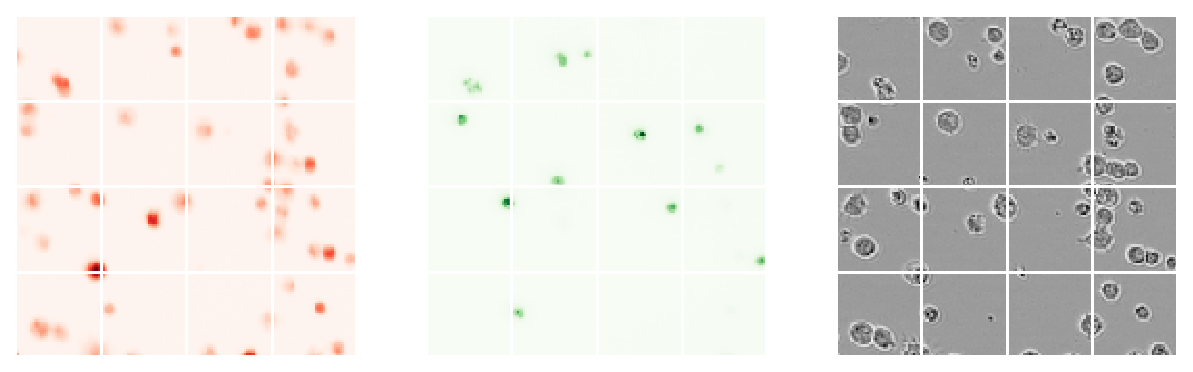
\includegraphics[width=\textwidth]{img/channels.pdf}
\caption{Aligned image channel crops ($200 \times200$px) marking living Raji cells in mCherry (left), dead cells in GFP (center), and phase contrast (right).}
\label{fig:cart:channels}
\end{figure}

Note the high volume of data: the cells are seeded to a total of up to $60000$ per well, with four wells per experiment type, each with four fields and $110$ time lapse frames. Coupled with the fluorescence annotations, this is, in principle, a veritable treasure trove of data for deep learning. Annotation by experiment is a promising strategy: a large ground truth can easily be collected and, in addition, the ``experimental ground truth'' is much more objective than a manual one. A similar strategy has already been applied to image segmentation (\cite{sadanandan2017automated}). This potentially overcomes the main bottleneck in leveraging deep learning models in such experiments. On the other hand, most cells fit inside a $14 \times 14$ pixel window (contrast this with the much higher resolutions of cells imaged in Part \ref{partI}). This low resolution proves to be a constraint in the analyses to come, and an engineering challenge for the models.

\subsection{Observations on the dataset}
\label{subsec:phenomena}

Even at the best of times it is highly advisable to perform an exploratory analysis of a dataset. This principle was put to get use in Chapter \ref{Chapter3}, as important insights were obtained that were carried through to Chapter \ref{Chapter4}. With the temporal dimension now thrown in, the CAR-T dataset proves to be highly dynamic, and becomes increasingly chaotic in time, in particular as the Raji B-cells undergo mitosis. Some notable phenomena observed in the experimental data are detailed presently. These prove to be influential factors in the methodological designs.

\subsubsection{Apoptotic cells acquire GFP}

Figure \ref{fig:dying_cell_frames} traces the death of a Raji cell in full fluorescence. One may observe some subtle morphological changes such as a reduction in size, as well as a change of texture, which remain visible on the phase contrast channel. The fluorescence, however, shows a clear accumulation of GFP fluorophores. Here, the average intensity of each fluorescent channel is measured in the cell region of interest and plotted over time in Figure \ref{fig:dying_cell_series}. The GFP signal rises for at least $10$ frames, corresponding to a $20$ hour period. The mCherry signal declines in time, seemingly in accordance with the quenching effect.

%
%\begin{figure}[h]
%\centering
%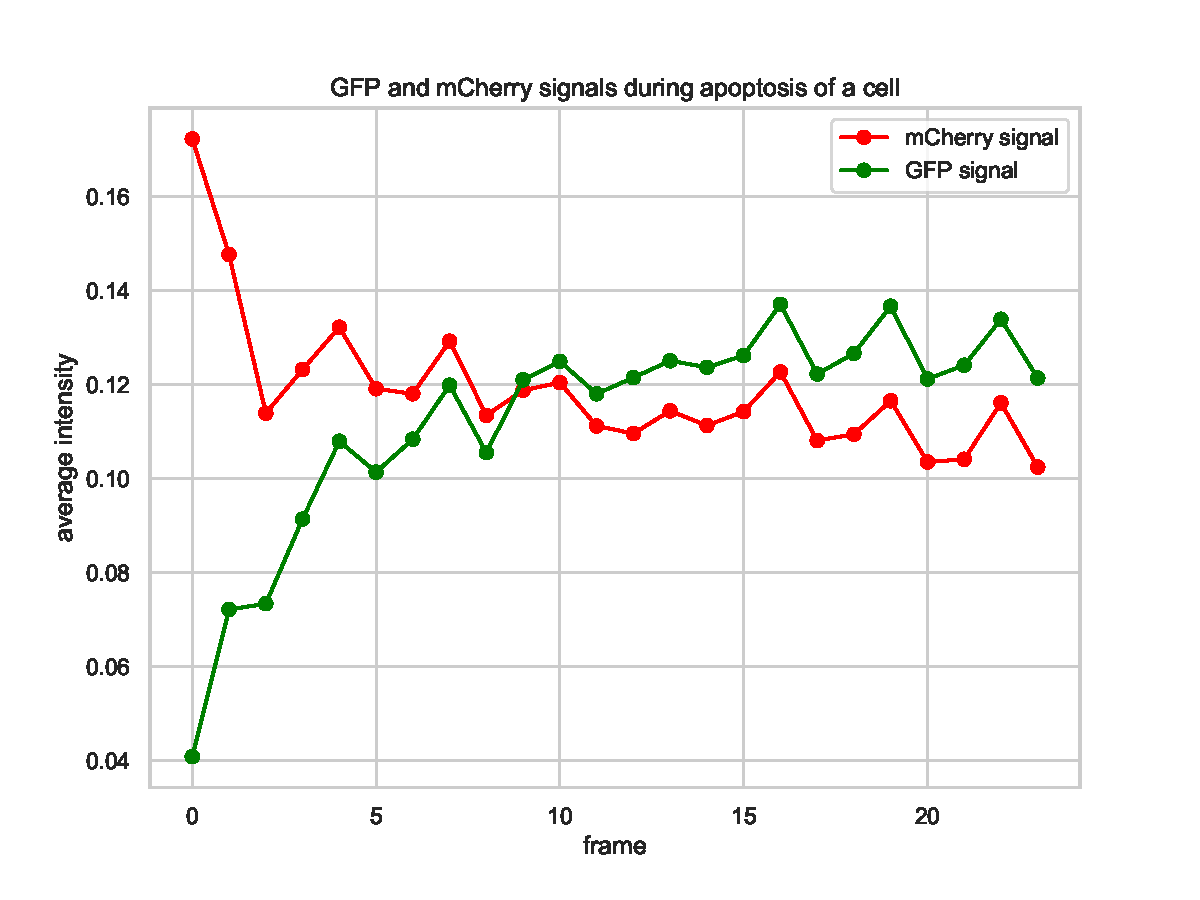
\includegraphics[width=0.85\textwidth]{img/dying_cell.pdf}
%\caption{Aligned image channel crops ($200 \times200$px) marking living Raji cells in mCherry (left), dead cells in GFP (center), and phase contrast (right).}
%\label{fig:dying_cell_graph}
%\end{figure}

\begin{figure*}[htb]
\centering
  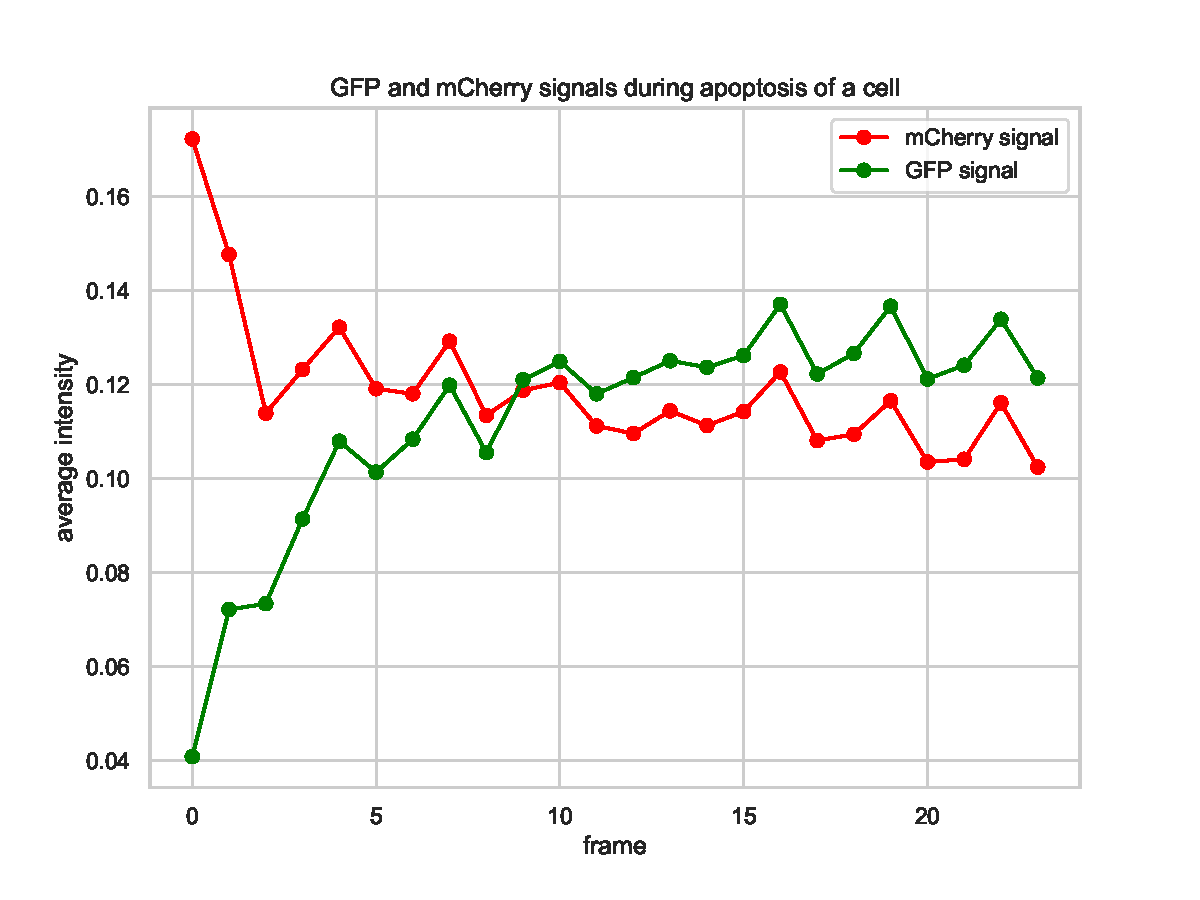
\includegraphics[width=\linewidth]{img/dying_cell.pdf}
  \caption{Tracking apoptosis of a Raji cell. GFP signal accumulates as a cell undergoes morphological changes (a)-(f).}
\label{fig:dying_cell_series}
\end{figure*}

%\begin{figure}[h!]%
%    \centering
%    \subfloat[\label{fig:dying_cell_frames_a}]{{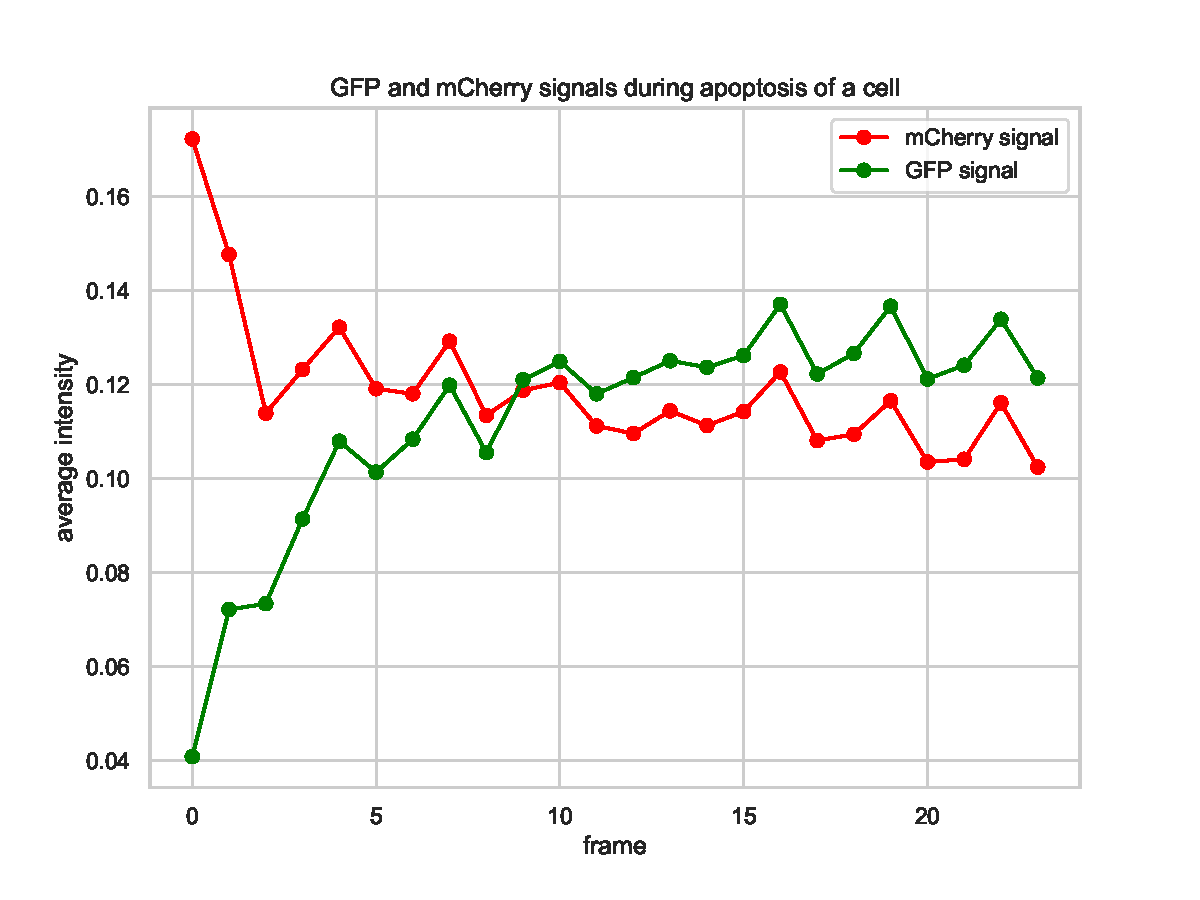
\includegraphics[width=0.9\textwidth]{img/dying_cell.pdf}}}
%	\qquad
%    \subfloat[\label{fig:dying_cell_frames_b}]{{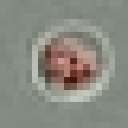
\includegraphics[width=.07\linewidth]{img/dying_cell_0000.png}}}%
%    \qquad
%    \subfloat[]{{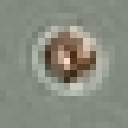
\includegraphics[width=.07\linewidth]{img/dying_cell_0001.png}}}%
%    \qquad
%    \subfloat[]{{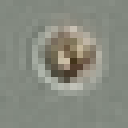
\includegraphics[width=.07\linewidth]{img/dying_cell_0002.png}}}%
%    \qquad
%    \subfloat[]{{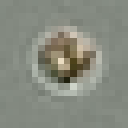
\includegraphics[width=.07\linewidth]{img/dying_cell_0003.png}}}%
%    \qquad
%    \subfloat[]{{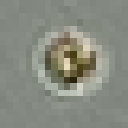
\includegraphics[width=.07\linewidth]{img/dying_cell_0004.png}}}%
%    \qquad
%    \subfloat[\label{fig:dying_cell_frames_g}]{{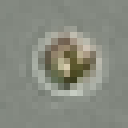
\includegraphics[width=.07\linewidth]{img/dying_cell_0005.png}}}%
%\caption{Tracking a mitotic event. The fluorescent turns green as a B cell undergoes morphological changes (a)-(f). This is reflected in a plot of intensity profiles (g).}
%\label{fig:dying_cell_frames}
%\end{figure}

\subsubsection{Proliferation of Raji cells leads to cell clumps}

Proliferation greatly complicates the task of counting cells, and influences the methods in the current chapter as well as the next. It is well known that Raji cells group to form clusters or ``clumps'' (\cite{epstein1966morphological}). Figure \ref{fig:mitosis_frames} shows a sequence of cropped frames centered on a proliferation of cells. From a handful of dispersed cells in the initial frame $(t = 50)$, cell division occurs in time $(t = 70)$, $(t = 80)$, $(t = 90)$, creating clusters of closely touching (or even overlapping) cells. Whatever methodological approach is taken, cell proliferation complexifies the detection and segmentation of individual cells as the image background can no longer be utilised to these ends. Whereas at first the cell contours are well-defined, the more the cells multiply, the less clear their separation, as cells begin to overlap.

\begin{figure}[h]%
    \centering
    \subfloat[$t=50$]{{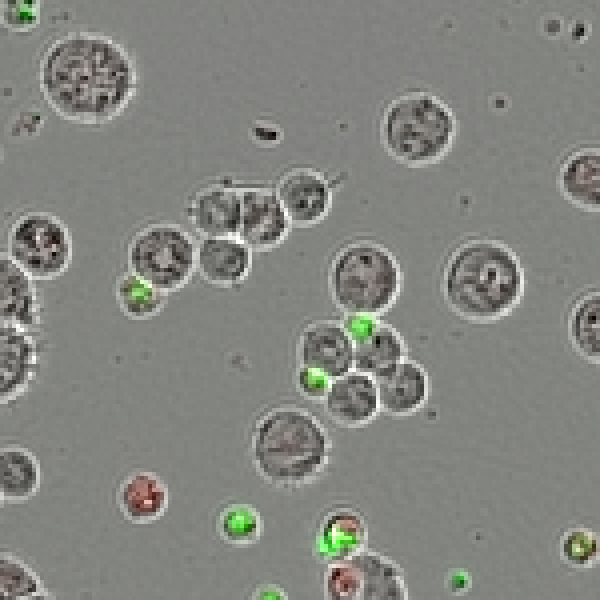
\includegraphics[width=.2\linewidth]{img/mitosis_25.png}}}%
    \qquad
    \subfloat[$t=70$]{{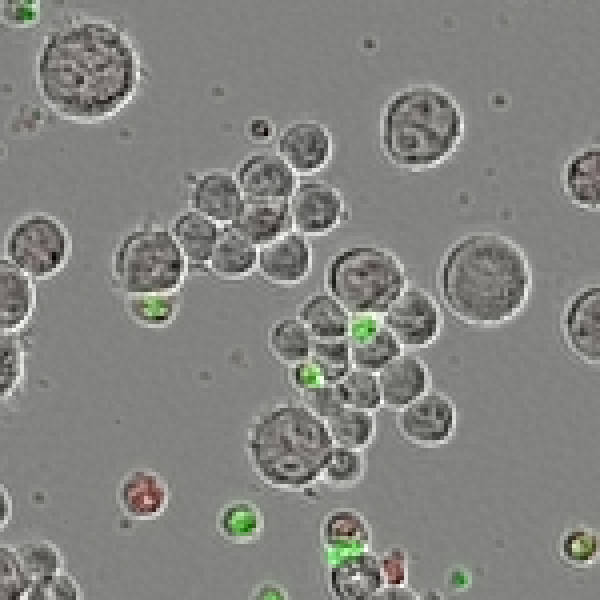
\includegraphics[width=.2\linewidth]{img/mitosis_35.png}}}%
    \qquad
    \subfloat[$t=80$]{{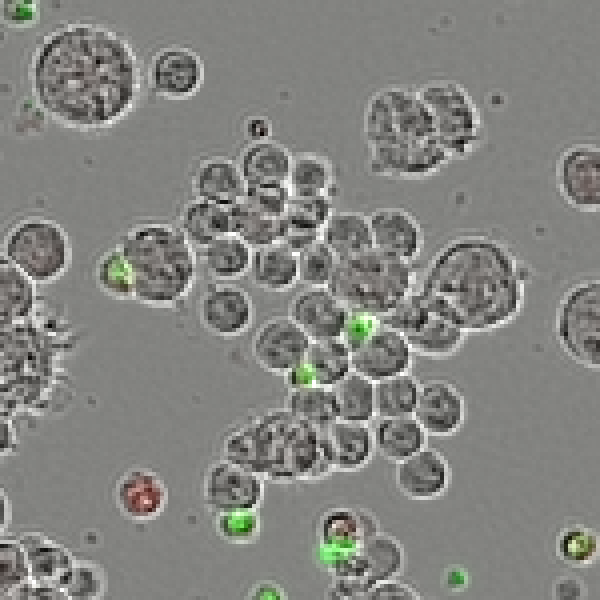
\includegraphics[width=.2\linewidth]{img/mitosis_40.png}}}%
	\qquad
    \subfloat[$t=90$]{{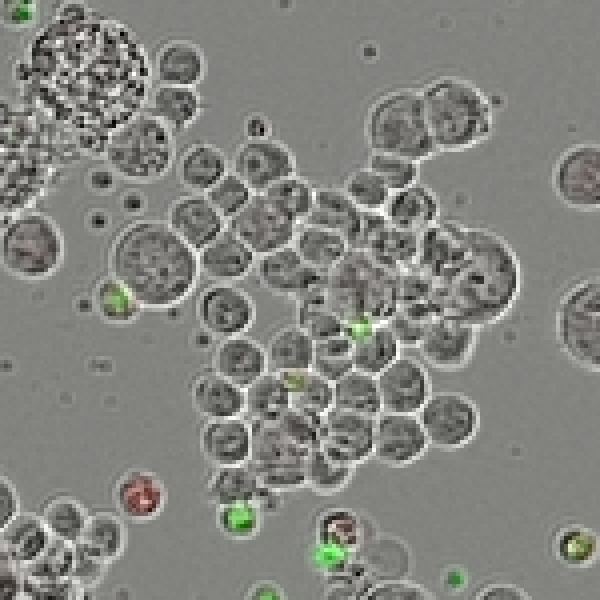
\includegraphics[width=.2\linewidth]{img/mitosis_45.png}}}%
\caption{Raji cell population over time. Proliferation generates cell clusters.}
\label{fig:mitosis_frames}
\end{figure}

\subsubsection{CAR-T cells create clusters of lysed target cells}

%\begin{figure}[h]%
%    \centering
%    \subfloat[]{{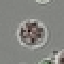
\includegraphics[width=.1\linewidth]{img/t_cell_21.png}}}%
%    \qquad
%    \subfloat[]{{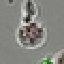
\includegraphics[width=.1\linewidth]{img/t_cell_22.png}}}%
%    \qquad
%    \subfloat[]{{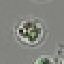
\includegraphics[width=.1\linewidth]{img/t_cell_46.png}}}%
%\caption{The processing of a test image: phase contrast input image (a); raw model bounding box predictions (b); non-maximum suppression post-processing (c); finally, for comparison, the corresponding full fluorescence image (d).}
%\label{fig:t_cell_frames}
%\end{figure}

With the inclusion of T cells, the picture becomes even more complicated. Figure \ref{fig:cluster_frames} shows a series of crops taken at $30$ hour intervals from well $B6$. T cells can here be seen as non-fluorescent objects with an elongated morphology. Their activities involve the killing of B cells, the lysed (fragmented) remains of which are shepherded into tight clusters of cellular matter. The formation and ultimate merging of several such clusters is observable in Figure \ref{fig:cluster_frames}. An example of a CAR-T cell latching onto a Raji antigen is also given, with the subsequent death of the Raji cell in Appendix \ref{fig:t_cell_latch}. From a modeling perspective, individual cells are impossible to discern from such entropic clusters, as the membrane that provides each cell with its identity has been lost. Perspectives for handling these cases are offered in Section \ref{sec:discussion_strategies}.

\begin{figure}[h]%
    \centering
    \subfloat[$t=0$]{{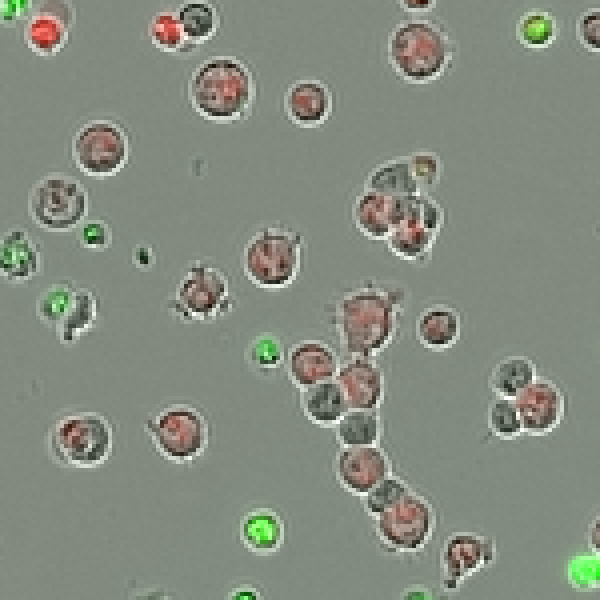
\includegraphics[width=.2\linewidth]{img/cluster_00.png}}}%
    \qquad
    \subfloat[$t=30$]{{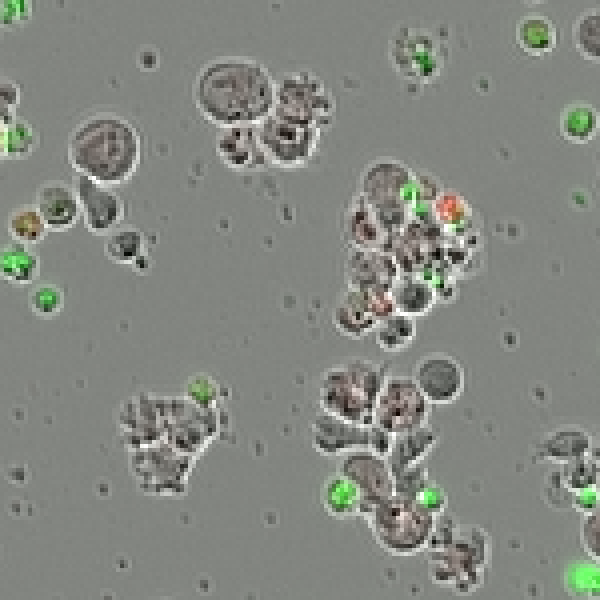
\includegraphics[width=.2\linewidth]{img/cluster_15.png}}}%
    \qquad
    \subfloat[$t=60$]{{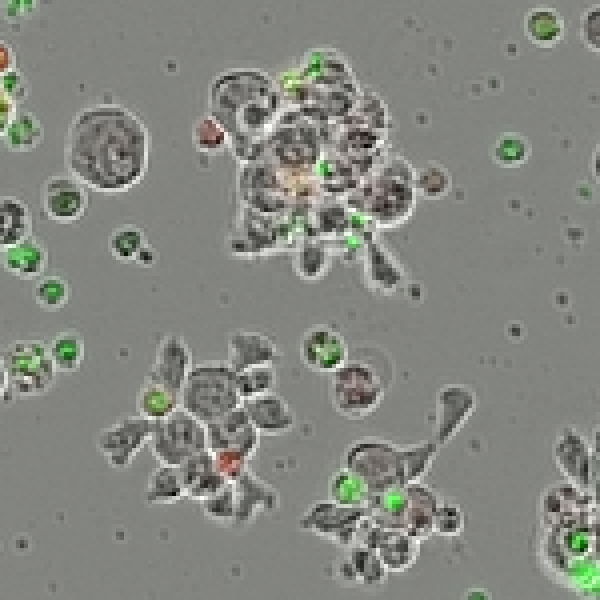
\includegraphics[width=.2\linewidth]{img/cluster_30.png}}}%
	\qquad
    \subfloat[$t=90$]{{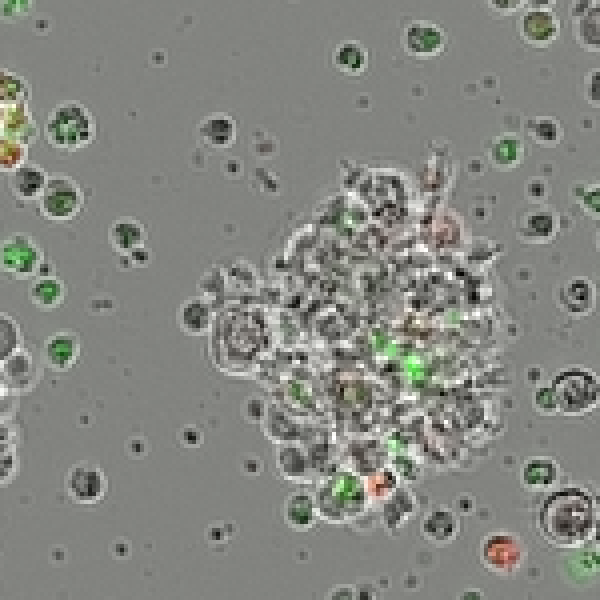
\includegraphics[width=.2\linewidth]{img/cluster_45.png}}}%
\caption{CAR-T cells (devoid of fluorescence) attack Raji B cells by latching onto Raji cell surface antigens and delivering cytotoxic chemicals. The induced lysis of the target Raji cells yields growing clusters of cellular matter.}
\label{fig:cluster_frames}
\end{figure}

%Phase contrast microscopy is a traditional microscopy technique developed in the 1930s that owes its popularity to both the simplicity of its experimental setup and a high contrast that is obtained by a smart arrangement of ring-shaped filters in the optical path. This high contrast, that does not require any particular sample preparation, allows to see structures in cells that are typically hidden in bright-field microscopy.
%
%In contrast, fluorescence microscopy allows to mark specific structures in cells with high contrast, either by immunofluorescence, live dyes or by genetic encoding of fluorescent reporters. Fluorescence microscopy is therefore the method of choice if we wish to highlight certain proteins of interest or the cellular compartments where these proteins localise. Importantly, this makes fluorescence microscopy particularly amenable for computational analysis. However, this high specificity and excellent contrast come at the price of visualising only partial information (only the marked proteins/cellular structures), of accepting a less physiological system (e.g. genetically modified cells) or more complicated experimental protocols (e.g. by the use of live dyes) and several experimental complications (such as fading dyes), in particular when imaging assays are performed over several days.

\subsection{Coping with fluorescent quenching}

Image-based screens of CAR-T cells, combining phase contrast and fluorescence microscopy, suffer from the gradual quenching of the fluorescent signal, making the reliable tracking of cell populations across time-lapse imagery difficult. We saw across Figures \ref{fig:dying_cell_series}, \ref{fig:mitosis_frames}, and \ref{fig:cluster_frames} evidence of the diminished mCherry (red) fluorescent signal in the later frames of the time lapse movies. In Figure \ref{fig:unnormalised_channels} we see how the distribution of total image fluorescence diminishes across time, regardless of well. Already, the quenching effect obfuscates the interpretation of the experiments by lab technicians. It is furthermore a complication for learning algorithms, as fluorescence becomes inversely correlated with the various cellular phenomena occurring in the latter stages of the experiment, for example: the dissemination of certain large cells due to cell growth, and the appearance of cell clusters due to cell proliferation and clustering, as illustrated above. Learning only on earlier frames, where the fluorescence is strongest, is unlikely to suffice. To mitigate the quenching effect, each pixel $x$ of image $\mathbf{x}$ is normalised to,

\begin{equation}
x' = \min(1, \frac{\bar{\mathbf{x}}_0}{\bar{\mathbf{x}}}\cdot\frac{x - \min(\mathbf{x})}{\text{perc}_{99}(\mathbf{x}) - \min(\mathbf{x})}),
\end{equation}

where $\bar{\mathbf{x}}_0$ and $\bar{\mathbf{x}}$ are the means of the initial image and the image to be normalised, and $\text{perc}_{99}$ returns the $99$th percentile intensity. Intensities below some small threshold $\tau$ are set to zero to remove background noise. Note that the potentially naive assumption is made that the loss of fluorescence is entirely due to quenching, and not the phenotypic changes in the population.


%\begin{figure}[h!]
%\centering
%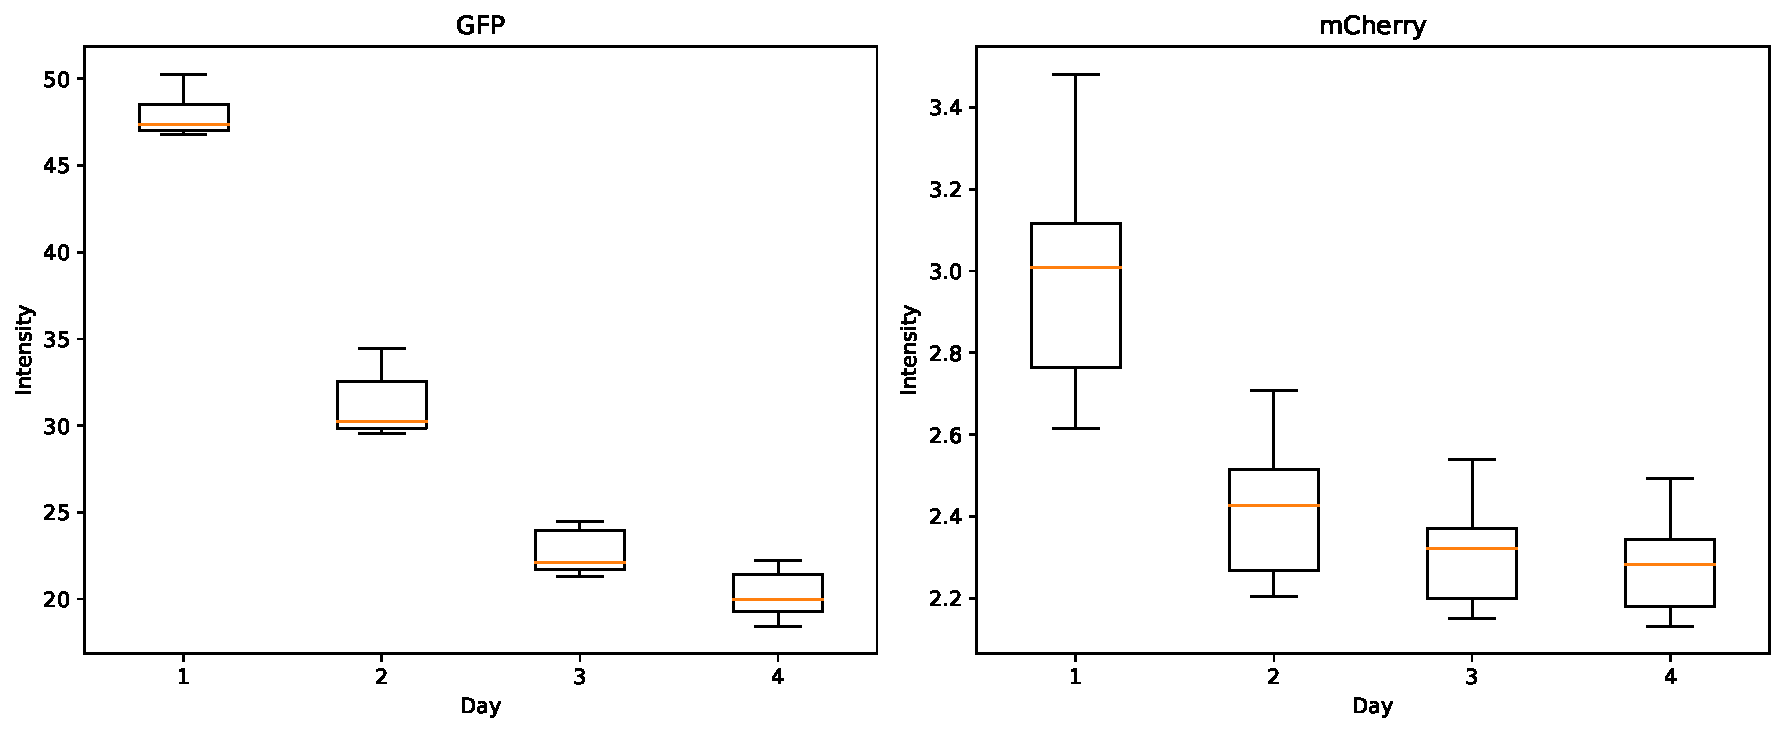
\includegraphics[width=0.85\textwidth]{img/unnormalised_channels.pdf}
%\caption{Comparison of average GFP (left) and mCherry (right) fluorescence measured across at different fields of view and compared $24$ hour intervals. One may observe the quenching effect of fluorescence over time, which occurs most rapidly in the first increment.}
%\label{fig:unnormalised_channels}
%\end{figure}

\begin{figure}%
    \centering
    \subfloat[GFP]{{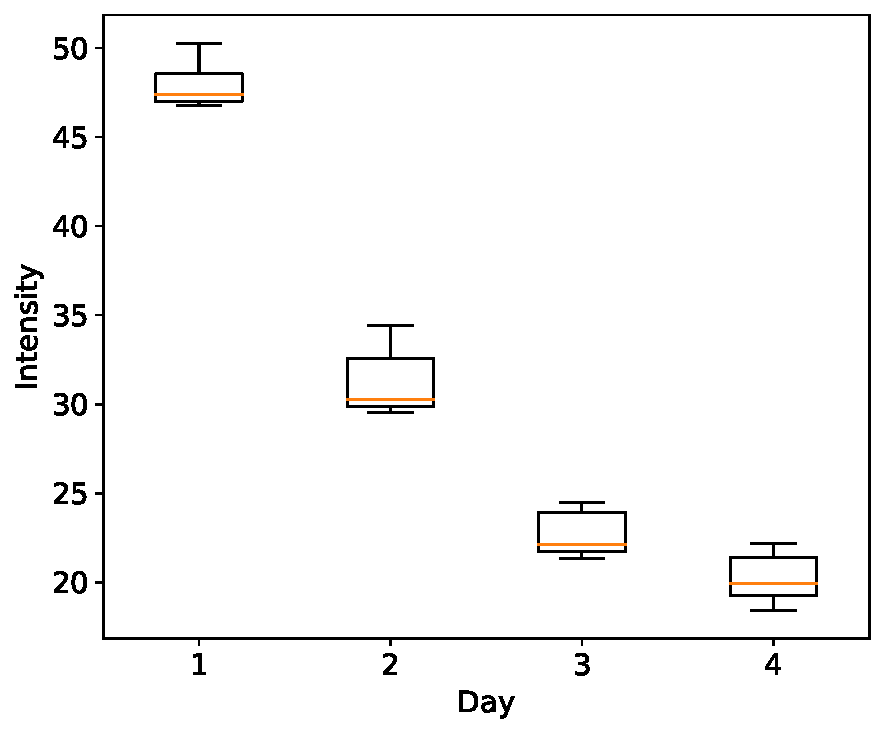
\includegraphics[width=.45\linewidth]{img/unnormalised_channels_gfp.pdf}}}%
    \qquad
    \subfloat[mCherry]{{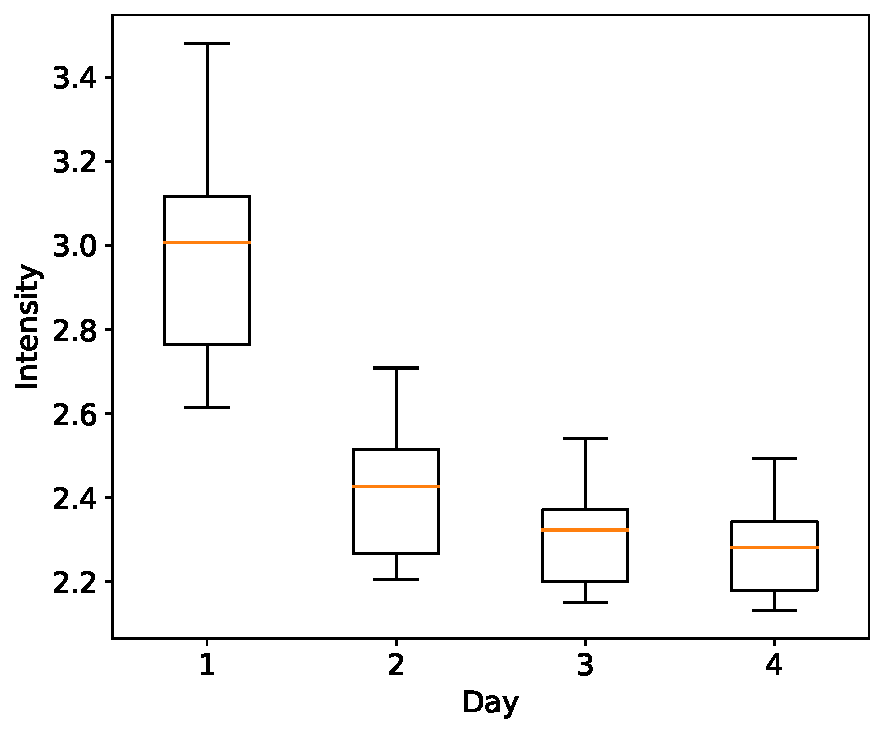
\includegraphics[width=.45\linewidth]{img/unnormalised_channels_mcherry.pdf}}}%
\caption{Comparison of average GFP (left) and mCherry (right) fluorescence measured across different fields of view at $24$ hour intervals. One may observe the quenching effect of fluorescence over time, which occurs most rapidly in the first increment.}
\label{fig:unnormalised_channels}
\end{figure}

%\begin{figure}[h!]
%\centering
%\includegraphics[width=\textwidth]{img/normalised_channels.pdf}
%\caption{Aligned image channel crops ($200 \times200$px) marking living Raji cells in mCherry (left), dead cells in GFP (center), and phase contrast (right).}
%\label{fig:gan_samples}
%\end{figure}

\section{Fluorescence prediction}
\label{sec:fluorescent_labeling}

In biological experiments pairing transmitted light and fluorescent signals, the fluorescence may often be largely inferred from the transmitted light image alone, as in \cite{christiansen2018silico}, \cite{ounkomol2018label}, and \cite{lee2018deephcs}. That is, given a pair $\mathbf{x}, \mathbf{y}$ of images from the transmitted light $X$ and fluorescence $Y$ image domains, the fluorescent labeler $F$ learns a mapping such that,

\begin{equation}
F(\mathbf{x}) \approx \mathbf{y}.
\end{equation}

Note that the prospects for predicting fluorescent will always depend on, among other things, the available image resolution. While \cite{ounkomol2018label} predicted fluorescent images of nucleoli, nuclear envelope, and microtubules from transmitted light images with a median Pearson correlation coefficient $r \geq 0.8$, ``painting'' other organelles such as desmosomes and Golgi apparatus worked far less well $r \leq 0.2$. In the experiments of this chapter, the relatively low resolution of cells must therefore be compensated by high-level morphological cues associating phenotype with fluorescence.

In the following, a family of models for performing fluorescence prediction of phase contrast images automatically are presented. The motivations of the system are twofold: firstly, it can be used as a visualisation tool; secondly, it may serve as an intermediate step in a cell counting system. Naturally, the quality of the latter function depends on that of the former.

\subsection{Image-to-image translation models}
\label{subsec:image_to_image}

Though not the only fluorescence labeler in the literature, the ``F-Net'', proposed by \cite{ounkomol2018label}, is a suitable baseline for the problem at hand, on the grounds that it is essentially a repurposed U-Net (\cite{ronneberger2015u}), a widely studied architecture. This architecture has a deep encoder-decoder structure, such as the autoencoders studied in Section \ref{subsubsec:dimensionality_reduction}, albeit fully convolutional, and with \emph{skip connections} concatenating each upsampling layer with its opposite downsampling layers. The full architecture specification is provided in Figure \ref{appendix:fnet}. The network is trained against the objective function,

\begin{equation}
\min_F \mathcal{L}_{L_2}(F) = \mathbb{E}_{\mathbf{x}, \mathbf{y}}[||\mathbf{y} - F(\mathbf{x})||_2^2],
\label{eq:l2_loss}
\end{equation}

that is, to minimise the expectation of mean square error over the distribution of input images $\mathbf{x}$ and target images $\mathbf{y}$, where $F : \mathbf{x} \to \mathbf{y}$ is the labeler network parameterised by a set of weights. The model is thus trained as a pixel-wise regressor. In the use cases to come, the input images are the phase contrast images, and the target images are the fluorescent channels. By default, the network is trained to predict a single fluorescent channel (as in \cite{ounkomol2018label}), producing one model per channel. Evidently, one could train a multi-task labeler to predict a multiplexed fluorescent output. Experiments with this approach did not yield a significant improvement in this setting, however.

Roughly speaking, the F-Net model is a special case of the image-to-image translation models proposed in \cite{isola2017image}. This family of \texttt{pix2pix} models may be formulated,

\begin{equation}
\min_G\max_D\mathcal{L}_{PIX}(D_{patch}, G) = \mathcal{L}_{CGAN}(D_{patch}, G) + \lambda\mathcal{L}_{1}(G),
\label{eq:pix2pix_loss}
\end{equation}

where $\mathcal{L}_{1}(G) = \mathbb{E}[||G(\mathbf{x}) - \mathbf{y}||_1]$ is mean absolute error with tuning hyperparameter $\lambda$ and $\mathcal{L}_{CGAN}$ is the conditional GAN (CGAN) objective (see Section \ref{subsec:conditional_gans_definition}),

\begin{align}\mathcal{L}_{CGAN}(D, G) = \mathbb{E}_{\mathbf{x} \sim p(\mathbf{x})}[\log D(\mathbf{x} | \mathbf{y})] + \mathbb{E}_{\mathbf{z} \sim p(\mathbf{z})}[\log(1 - D(G(\mathbf{z} | \mathbf{y})))],
\end{align}

where $D$ is the discriminator and $G$ is the generator, equivalent to $F$ in all respects aside from it using a hyperbolic tangent ($\tanh$) function in the output layer (as is conventional for DCGANs, see Section \ref{subsec:dcgan_definition}) rather than a linear one. The variable $\mathbf{z}$ refers to the generator's noise input. In the image-to-image setting, the discriminator network is a fully-convolutional network denoted ``PatchGAN'' (see Appendix \ref{appendix:patch_gan} for an implementation),

\begin{equation}
d_{patch} : X, Y \to [0, 1]^{h\times w},
\end{equation}

producing an $h\times w$ grid of outputs rather than a single neuron, with each grid element critiquing an overlapping region of the input image. The grid of outputs are then averaged to give the discriminator,

\begin{equation}
D_{patch}(\mathbf{x}, \mathbf{y}) = \frac{1}{hw}\sum_{i=0}^h\sum_{j=0}^w d_{patch}(\mathbf{x}, \mathbf{y})_{ij}.
\end{equation}

In practice, the conditioning is implemented as a channel-wise concatenation of condition image $\mathbf{x}$ and the target $\mathbf{y}$. \cite{isola2017image} make the insightful observation, however, that a GAN learns its own loss function via the discriminator, which penalises ``unrealistic'' images. As such, it is an infinitely flexible methodology and the discriminator $D$ can be understood to act as an adaptive loss function, analagous to the way features are learned and optimised for the task of classification within the layers of a deep classifier. The choice of $L_1$ over an $L_2$ auxiliary loss is based on the empirical observation that $L_2$ leads to blurry results, something observe presently. The \texttt{pix2pix} system has been demonstrated to be effective on a wide range of image-to-image translation problems. Just as with U-Net, they can achieve impressive results, while trained on a relatively small number of images.

In addition to the above, the F-Net $F$ is also trained against a mean absolute error loss,

\begin{equation}
\min_F\mathcal{L}_{L_1}(F) = \lambda\mathcal{L}_{1}(F).
\label{eq:l1_loss}
\end{equation}

All models (Equations \ref{eq:l2_loss}, \ref{eq:pix2pix_loss}, and \ref{eq:l1_loss}) were trained on $1120$ non-overlapping $256\times256$px phase contrast crops paired with fluorescence crops selected from the first $14$ fields of view from each experimental setting separately (rows A and B of the plate). Recall each fluorescent channel is trained on separately, producing separate models. The cropping strategy sampled from the first frame of each $24$-hour window, for the first $96$ hours of each time lapse movie. This strategy was adopted to maximise the available variation in the training data, without losing too much to the fluorescent quenching effect of later frames, while at the same time retaining the convenience of keeping all images in memory. Validation and testing was performed according to the same strategy on independent fields A06\_03 and A06\_04. Batches of a single image were sampled randomly and all models were trained with the Adam optimiser with $(\beta_0, \beta_1) = (0.5, 0.999)$ and maximum learning rate $2\times10^{-4}$.

\subsection{Results}

In practice, a fluorescence prediction ought to be considered good if the placement of its predictions are accurate, even if it does not match the ground truth intensities accurately. For this reason \cite{ounkomol2018label} propose an evaluation based on the Pearson correlation coefficient (PCC),

\begin{align}
r = \frac{\sum (x - \bar{x})(y - \bar{y})}{\sqrt{\sum (x - \bar{x})^2\sum (y - \bar{y})^2}},
\end{align}

over all pixels $x$ in the prediction and $y$ in the test image. Figure \ref{fig:pix2pix_pcc} compares the average PCC correlation across all test images for each of the three models and each mode (GFP, mCherry) on the Raji-only experiments. The best overall performance comes from the $L_2$ model with mean $0.7617$ and standard deviation $0.1049$ for mCherry labeling, and mean $0.6163$ and standard deviation $0.0931$ for GFP. The pix2pix system performs at mean $0.7573$ and standard deviation $0.0814$ for mCherry, and mean $0.5848$ and standard deviation $0.0972$ for GFP. Finally, the $L_1$ model performs at mean $0.7720$ and standard deviation $0.0727$ for mCherry, and $0.5115$ and standard deviation $0.1099$ for GFP. Paradoxically, the $L_2$ model appears, by inspection, to generate worse results, with a significant amount of fluorescent ``spillage'' and blur effects. However, this noise can be removed with a simple thresholding operation. The pix2pix outputs look initially sharper, but ultimately fail more often to apply fluorescence where it counts, leading to a greater number of false negatives. On the other hand, it is also clear that the $L_2$ and $L_1$ models exhibit a greater degree of mode collapse than the pix2pix model, which necessarily varies its fluorescent prediction to continuously fool the discriminator.

%\begin{figure}[h!]
%\centering
%\includegraphics[width=0.65\textwidth]{img/pix2pix_mse.pdf}
%\caption{Aligned image channel crops ($200 \times200$px) marking living Raji cells in mCherry (left), dead cells in GFP (center), and phase contrast (right).}
%\label{fig:unnormalised_channels}
%\end{figure}

\begin{figure}[h!]
\centering
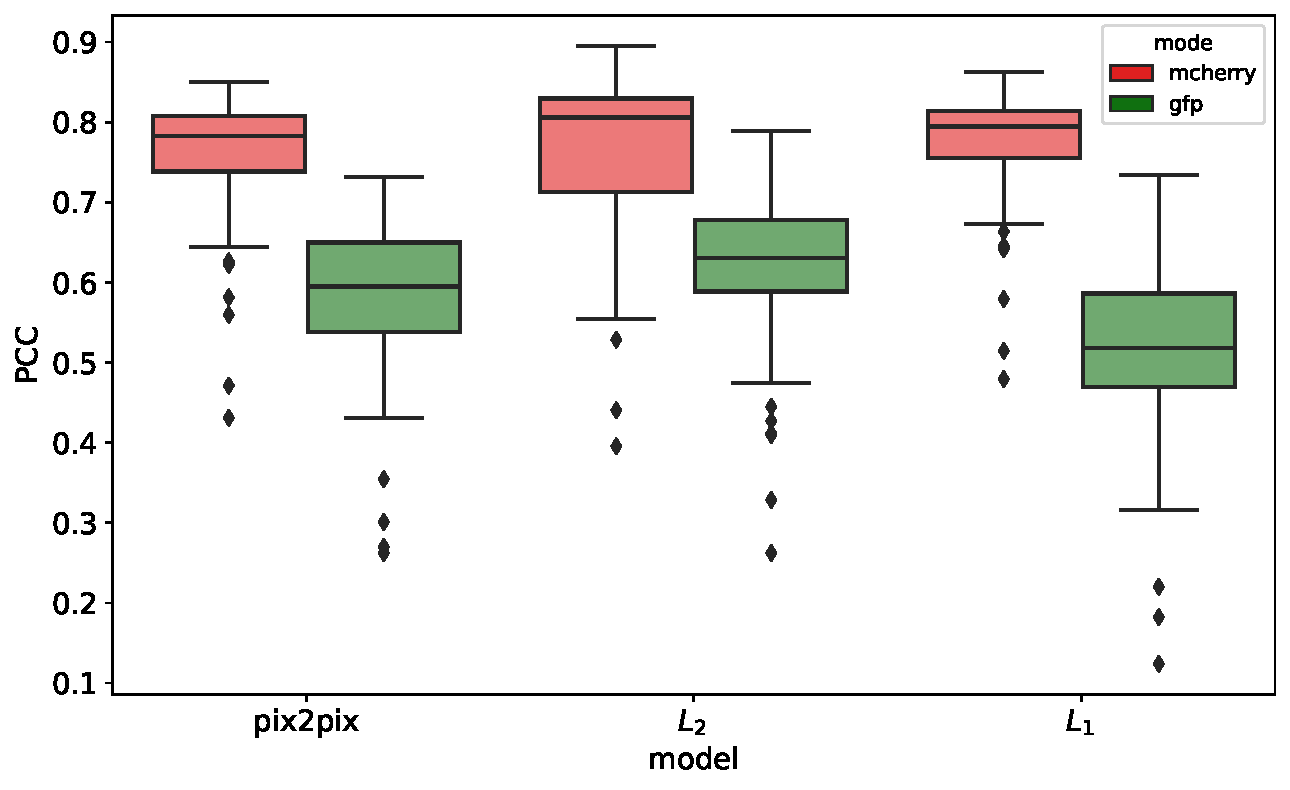
\includegraphics[width=0.85\textwidth]{img/pix2pix_pcc.pdf}
\caption{Pearson correlation coefficients for outputs of three fluorescent labelers, for both mCherry and GFP fluorescence prediction, measured over $80$ test images.}
\label{fig:pix2pix_pcc}
\end{figure}

\subsubsection{Visualising full fluorescence outputs}

An important qualitative test is to visualise the joint model outputs in full fluorescent colour, as well as in time lapse. To produce an appealing output, a ``camera shake'' effect of the plate moving inside the microscope must be corrected. Between successive frames, this is usually no more than $10 \mu m$, corresponding to about $7$px, in any direction. The necessary correction $(\delta x, \delta y)$ is found frame by frame by brute force over a suitable range of offsets. Fortunately, the Raji cells do not move much over time, and therefore the right offset can be found as the one that minimises the squared error between the frames. The images are each cropped slightly to account for the extents of the cumulative displacements in each direction caused by the shake. This tends to be a small amount, apparently with the camera displacements occurring around a fixed center of mass. Lastly, the frames of the fluorescent channels are corrected by the same offsets discovered in the phase contrast.

The RGB pixel at position $(i, j)$ of each full fluorescence image $I$ is set as,

\begin{equation}
I_{ij} = [M_{ij} + P_{ij}, G_{ij} + P_{ij}, P_{ij}],
\end{equation}

where $M$ is the mCherry channel, $G$ is the GFP channel, and $P$ is the phase contrast image. The values are further clipped to the range $[0, 1]$. Figures \ref{fig:full_colour_raji} and \ref{fig:full_colour_t_cells} compare synthesised images combined from the respective \texttt{pix2pix} fluorescent labelers to the corresponding ground truth fluorescence. The errors are manifest, yet the models do a fine job of discerning cell types, implicit in their application of GFP over dead Raji cells in the Raji-only experiment (Figure \ref{fig:full_colour_raji}) and its leaving T cells unlabelled in the full CAR-T experiment (Figure \ref{fig:full_colour_t_cells}), as per the logic of Equation \ref{eq:fuzzy_logic}. The predicted fluorescence intensity levels also closely approximate those of the ground truth. Nevertheless, it should be noted that the the mutual information between fluorescence intensity and phase contrast morphology may ultimately be too small to always guarantee an accurate prediction of intensity. For this reason, one must accept, for example, that certain dead cells appear more yellow than green, and vice versa. One possible extension of this work could be to incorporate time information into the prediction, which might alleviate this effect. Ultimately, however, it may be confirmed in the broader picture, that the fluorescent prediction is a success as a visualisation tool, at least for the earlier frames of the time lapse, and it ought now be considered how to incorporate it into a practicable tool for experimental use.

Full $110$-frame time lapse movies comparing prediction (left) and ground truth full fluorescence (right) may be found online: Raji-only ($256\times256$px)\footnote{https://jcboyd.github.io/assets/car-t-videos/raji\_target/256.mp4}, Raji-only ($512\times512$px)\footnote{https://jcboyd.github.io/assets/car-t-videos/raji\_target/512.mp4}, full CAR-T ($256\times256$px)\footnote{https://jcboyd.github.io/assets/car-t-videos/CAR\_June/256.mp4}, and full CAR-T ($512\times512$px)\footnote{https://jcboyd.github.io/assets/car-t-videos/CAR\_June/512.mp4}.

\begin{figure}%
    \centering
    \subfloat[Prediction ($t = 0$)]{{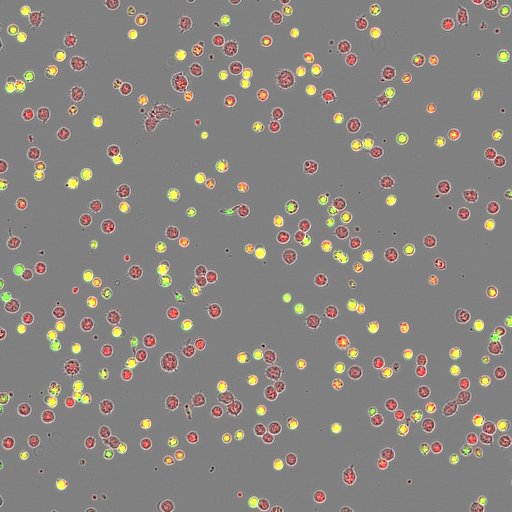
\includegraphics[width=.45\linewidth]{img/full_colour_0001a.png}}}%
    \qquad
    \subfloat[Ground truth ($t = 0$)]{{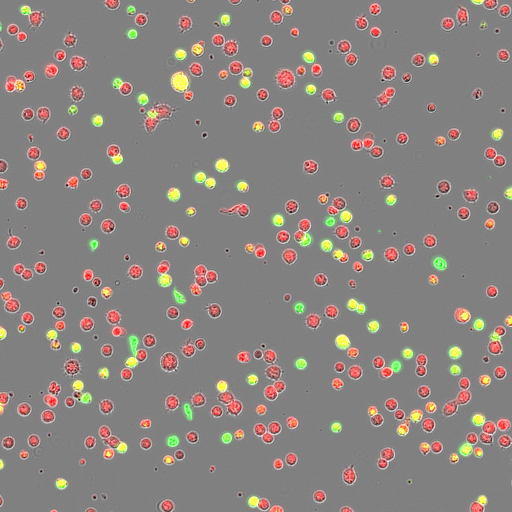
\includegraphics[width=.45\linewidth]{img/full_colour_0001b.png}}}%
    \qquad
    \subfloat[Prediction ($t = 48$)]{{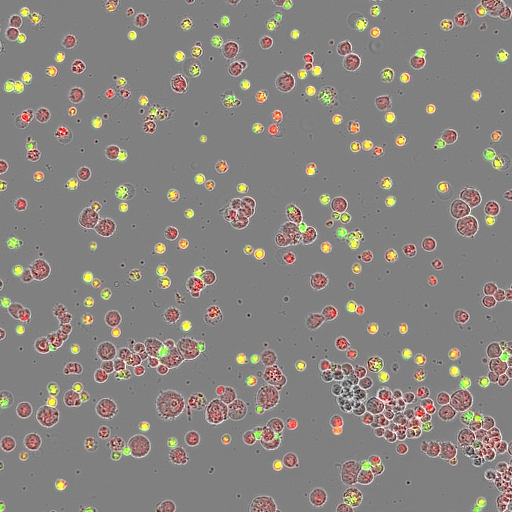
\includegraphics[width=.45\linewidth]{img/full_colour_0048a.png}}}%
    \qquad
    \subfloat[Ground truth ($t = 48$)]{{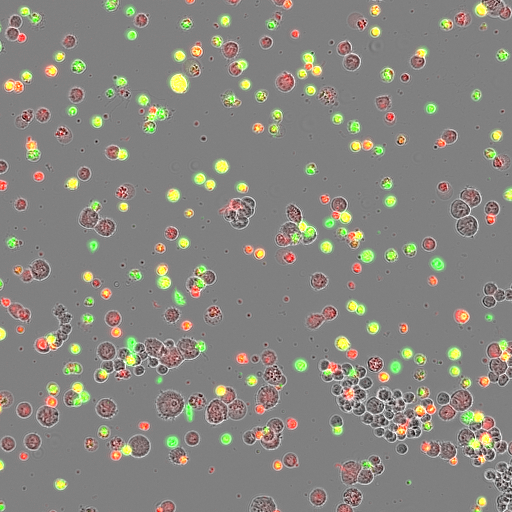
\includegraphics[width=.45\linewidth]{img/full_colour_0048b.png}}}%
\caption{Full fluorescence for indicative ($512 \times 512$px) crop from an Raji-only experiment. Columns distinguish fluorescent labeler predictions (left) and ground truth (right); rows distinguish times an early frame ($t=0$) (top) and a later one ($t=48$) (bottom).}
\label{fig:full_colour_raji}
\end{figure}

\begin{figure}%
    \centering
    \subfloat[Prediction ($t = 0$)]{{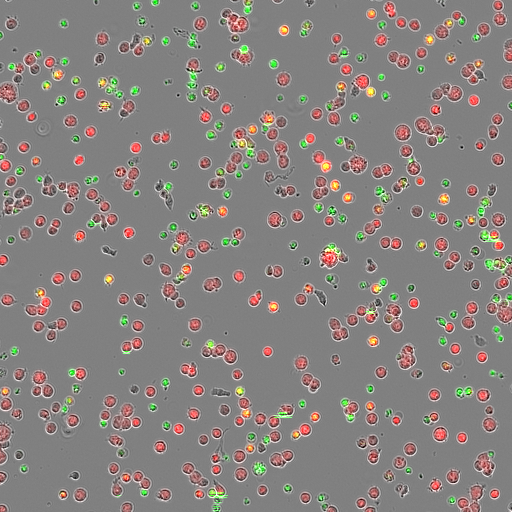
\includegraphics[width=.45\linewidth]{img/full_colour_t_0000a.png}}}%
    \qquad
    \subfloat[Ground truth ($t = 0$)]{{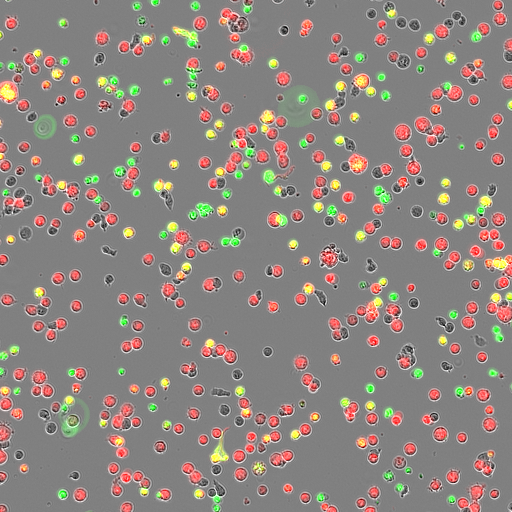
\includegraphics[width=.45\linewidth]{img/full_colour_t_0000b.png}}}%
    \qquad
    \subfloat[Prediction ($t = 40$)]{{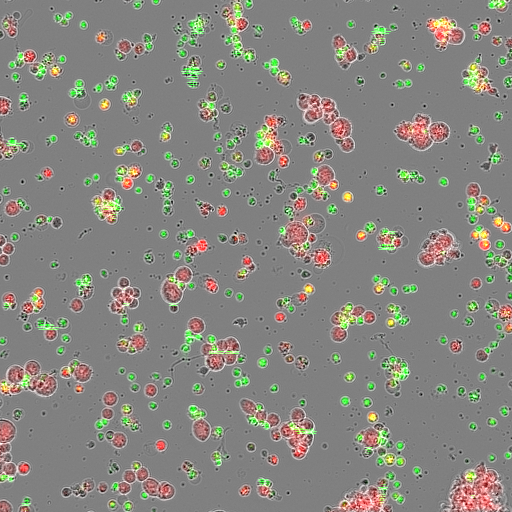
\includegraphics[width=.45\linewidth]{img/full_colour_t_0040a.png}}}%
    \qquad
    \subfloat[Ground truth ($t = 40$)]{{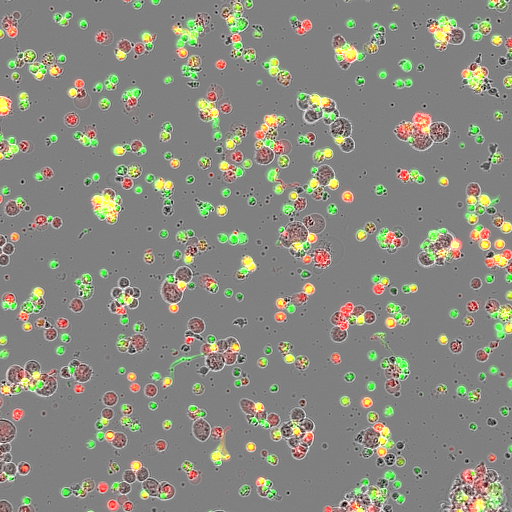
\includegraphics[width=.45\linewidth]{img/full_colour_t_0040b.png}}}%
\caption{Full fluorescence for indicative ($512 \times 512$px) crop from a CAR-T experiment. Columns distinguish fluorescent labeler predictions (left) and ground truth (right); rows distinguish times an early frame ($t=0$) (top) and a later one ($t=40$) (bottom).}
\label{fig:full_colour_t_cells}
\end{figure}

%\begin{figure}%
%    \centering
%
%\caption{Put your caption here}
%\label{fig:full_colour_0048}
%\end{figure}

%\begin{figure}[ht]
%\begin{subfigure}{.5\textwidth}
%  \centering
%  % include first image
%  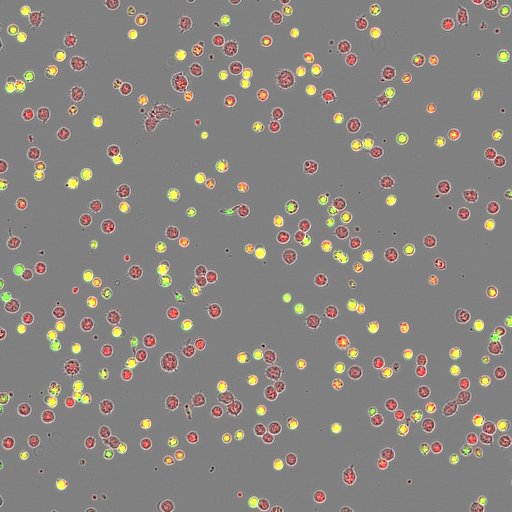
\includegraphics[width=.8\linewidth]{img/full_colour_0001a.png}  
%  \caption{Put your sub-caption here}
%  \label{fig:sub-first}
%\end{subfigure}
%\begin{subfigure}{.5\textwidth}
%  \centering
%  % include second image
%  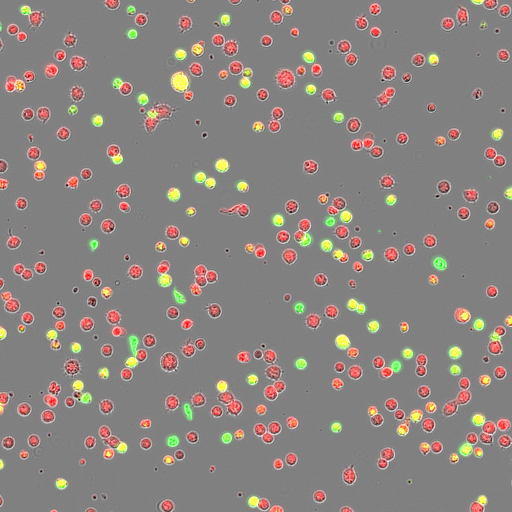
\includegraphics[width=.8\linewidth]{img/full_colour_0001b.png}  
%  \caption{Put your sub-caption here}
%  \label{fig:sub-second}
%\end{subfigure}
%\caption{Put your caption here}
%\label{fig:full_colour_0001}
%\end{figure}
%
%\begin{figure}[ht]
%\begin{subfigure}{.5\textwidth}
%  \centering
%  % include first image
%  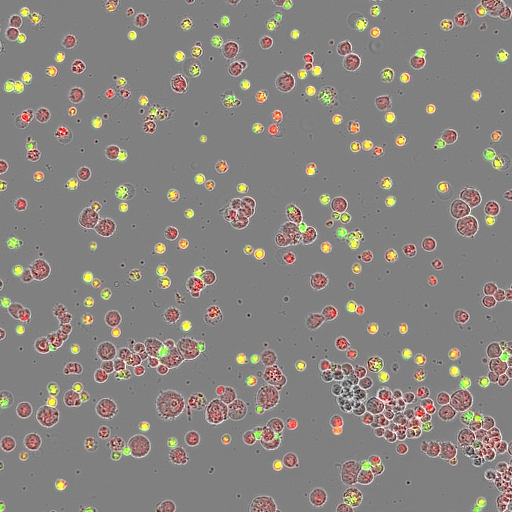
\includegraphics[width=.8\linewidth]{img/full_colour_0048a.png}  
%  \caption{Put your sub-caption here}
%  \label{fig:sub-first}
%\end{subfigure}
%\begin{subfigure}{.5\textwidth}
%  \centering
%  % include second image
%  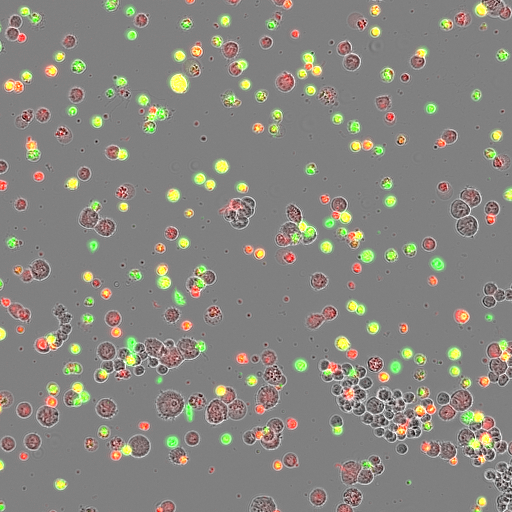
\includegraphics[width=.8\linewidth]{img/full_colour_0048b.png}  
%  \caption{Put your sub-caption here}
%  \label{fig:sub-second}
%\end{subfigure}
%\caption{Put your caption here}
%\label{fig:full_colour_0048}
%\end{figure}

\subsection{Bridging the gap to cell detection}

In the present problem context, it is of interest to derive a quantitative profile from live cell imaging data. While effective as a visualisation tool, fluorescent prediction only goes partway towards a full quantification of the phase contrast contents. Consider sample outputs for densely clustering cells, given in Figure \ref{fig:in_silico_problems}. Here we can see how the task of counting cells is far from complete following fluorescence prediction, with dense ``clouds'' of fluorescence corresponding to masses of cells. One can imagine all sorts of \emph{post hoc} solutions for disambiguating these fluorescent clouds.

\begin{figure}%
    \centering
    \subfloat[Phase contrast input]{{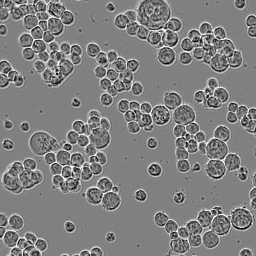
\includegraphics[width=.45\linewidth]{img/example_1_pc.png}}}%
    \qquad
    \subfloat[mCherry fluorescent output]{{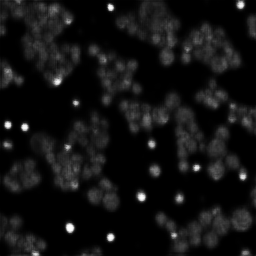
\includegraphics[width=.45\linewidth]{img/example_1_mcherry.png}}}%
    \qquad
    \subfloat[Phase contrast input]{{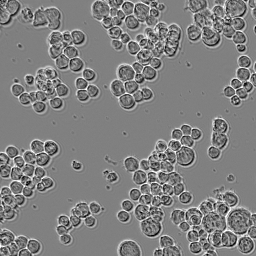
\includegraphics[width=.45\linewidth]{img/example_2_pc.png}}}%
    \qquad
    \subfloat[mCherry fluorescent output]{{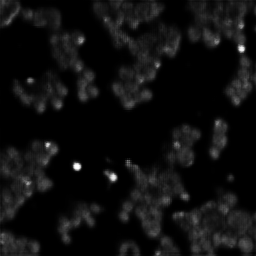
\includegraphics[width=.45\linewidth]{img/example_2_mcherry.png}}}%
\caption{Fluorescent labeler outputs produce dense clouds of mCherry fluorescence for two manually selected phase contrast inputs. These outputs may be difficult to disambiguate.}
\label{fig:in_silico_problems}
\end{figure}

\subsubsection{Blob detection for disambiguating fluorescent labels}

As Raji cells have a consistent size and simply, circular geometry, one approach to counting individual cells from the fluorescence prediction outputs is with \emph{blob detection}. A simple approach to blob detection is with a Laplacian of Gaussian (LoG) filter. That is,

\begin{equation}
\Delta G_\sigma(x, y) * I(x, y) = [\nabla_{xx}G_\sigma(x, y) + \nabla_{yy}G_\sigma(x, y)] * I(x, y),
\end{equation}

where $\Delta$ is the Laplacian operator (sum of second partial derivatives), $G_\sigma$ is a Gaussian filter with standard deviation $\sigma$ and $I$ is an image. Blobs distribute intensities in a Gaussian-like way, and the Gaussian pre-filter smooths the image. The second derivative of a Gaussian has a minimum in the center of the bell curve, thus marking the center of the blob. The maxima detected in the resultant image are the detected blobs. Usually the filter is performed over a range of scales, from which are chosen the maxima.

In practice, the tunable parameters for LoG blob detection are the range of standard deviations $\{\sigma_i\}$ to test for (corresponding to the anticipated size range) and a threshold $\theta$ on the minimum permissible intensity. These were tuned by hand in an example of this approach to blob detection of fluorescent outputs provided in Figure \ref{fig:blob_detection}.

This simple approach to blob detection, however, is found to not suffice for cases such as in in Figure \ref{fig:in_silico_problems}. While some system could surely be devised to infer the number of cells from a mass of flouroscence, in the following section we will see an alternative approach based on the fundamentally distinct methodology of object detection, which makes counting cells a primary objective.

\section{Object detection system}
\label{sec:object_detection_system}

\emph{This section contains an extended version of a paper published in the proceedings of the International Symposium for Biomedical Imaging in 2020.}

We found in the previous section a limitation on the scope of fluorescent prediction for counting cells. This brings us back to a more conventional high content analysis (HCA). In Chapter \ref{Chapter4} the concern was with generating a phenotypic profile that characterised a drug effect, potentially with uninterpretable intermediate features. In the present context, we are concerned with the more comprehensible task of counting cell types in time. Note that this task conforms to the conventional pipeline (see Section \ref{subsec:HCA}). In particular, the dimensionality reduction step will be fulfilled by the attribution of a cell type,

\begin{equation}
\mathbf{z} = f(\mathbf{x}),
\end{equation}

where $\mathbf{z} \in \{0, 1\}^K$ and $\sum_{k=0}^K z_k = 1$ for $K$ the number of cell classes, that is, $\mathbf{z}$ is one-hot, for extracted cell features $\mathbf{x}$, and cell classifier $f$. The cell population is then summarised by aggregation as a simple summation or average, giving the number or proportion of cells per cell class respectively in the phenotypic profile,

\begin{equation}
\mathbf{p} = \frac{1}{N}\sum_{i=1}^N f(\mathbf{x}_i).
\end{equation}

As we shall see, in this section the first three stages of the HCA pipeline are achieved by a single neural network.

A phenotypic profile of this nature summarises a single image frame. However, we are interested in summarising a full time lapse movie. Therefore, our aim is to create a set of such count profiles, 

\begin{equation}
\mathbb{P} = \{\mathbf{p}_i\}_{i=0}^{T},
\end{equation}

where $\mathbf{p}_i \in \mathbb{R}^K$ for $K$ classes is the $i$th profile in a series of $T$ frames. This ordered set amounts to a set of $K$ time series, one per class, of length $T$, and is the final output in Section \ref{subsec:object_detection_results}.

Section \ref{subsec:object_detection_data} describes an acquisition and preprocessing pipeline for an experimentally-generated ground truth with which to train the detection system. Section \ref{subsec:training} specifies this system, and Section \ref{subsec:object_detection_results} we describe our evaluation methodology and report model performance on two manually annotated datasets. This section considers only the Raji-only experimental setting. Note, however, that the methodology should naturally extend to the full CAR-T setting also.

\subsection{Experimentally-generated ground truth}
\label{subsec:object_detection_data}

Our pipeline (see Figure \ref{fig:pipeline_ground_truth}) begins by applying a Gaussian filter (tuned to $\sigma = 2$) to the phase contrast image. We then segment cells by subtracting a background image formed with a mean filter of diameter $19$px, before clipping to zero as in \cite{walter2010automatic}. We fill object holes with a morphological reconstruction by erosion and use a morphological opening to remove small details. An example of this pipeline depicted in Figure \ref{fig:ground_truth_pipeline_example}. We further filter objects outside a reasonable size range ($< 6 \times 6$px $\approx 50 \mu m^2$, determined by ranking cell areas), as these tend to be dust and other non-cellular particles on the well surface. An Otsu threshold on the distribution of averaged GFP signal per cell is then used to allocate a class (living/dead) for each connected component (see Figure \ref{fig:gfp_bimodal}). To train our object detector (Section \ref{subsec:training}), we also randomly sample background crops from the images, allowing for partial overlaps with cells.

\tikzstyle{block} = [rectangle, draw, fill=blue!20, node distance=2.5cm,
    text width=3.5em, text centered, rounded corners, minimum height=3em]
\tikzstyle{line} = [draw, -latex']

\begin{figure}
\centering
\begin{tikzpicture}[node distance=0.5cm, text width=3em, minimum height=3em, font=\tiny]
    % Place nodes
    \node [block, fill=red!20] (green) {GFP};
    \node [block, left of=green, fill=red!20] (pc) {Phase contrast};
    \node [block, right of=green, fill=red!20] (red) {mCherry};

	\node [block, below of=green] (fill) {Fill holes};
	\node [block, left of=fill] (bs) {Background subtraction};
	\node [block, left of=bs] (prefilter) {Prefilter};
	\node [block, right of=fill] (features) {Extract features};
	\node [block, right of=features] (classes) {Assign classes};
    % Draw edges
    \path [line] (pc) -- (prefilter);
    \path [line] (prefilter) -- (bs);
    \path [line] (bs) -- (fill);
	\path [line] (fill) -- (features);
%    \path [line] (fill) -- (label);
%    \path [line] (label) -- (features);
    \path [line] (features) -- (classes);
	\path [line] (green) -- (features);
	\path [line] (red) -- (features);
\end{tikzpicture}
\caption{Pipeline for automatic construction of ground truth for training object detection system. Basic image processing steps indicated in blue, image inputs indicated in red.}
\label{fig:pipeline_ground_truth}
\end{figure}

\begin{figure}[htb]
\centering
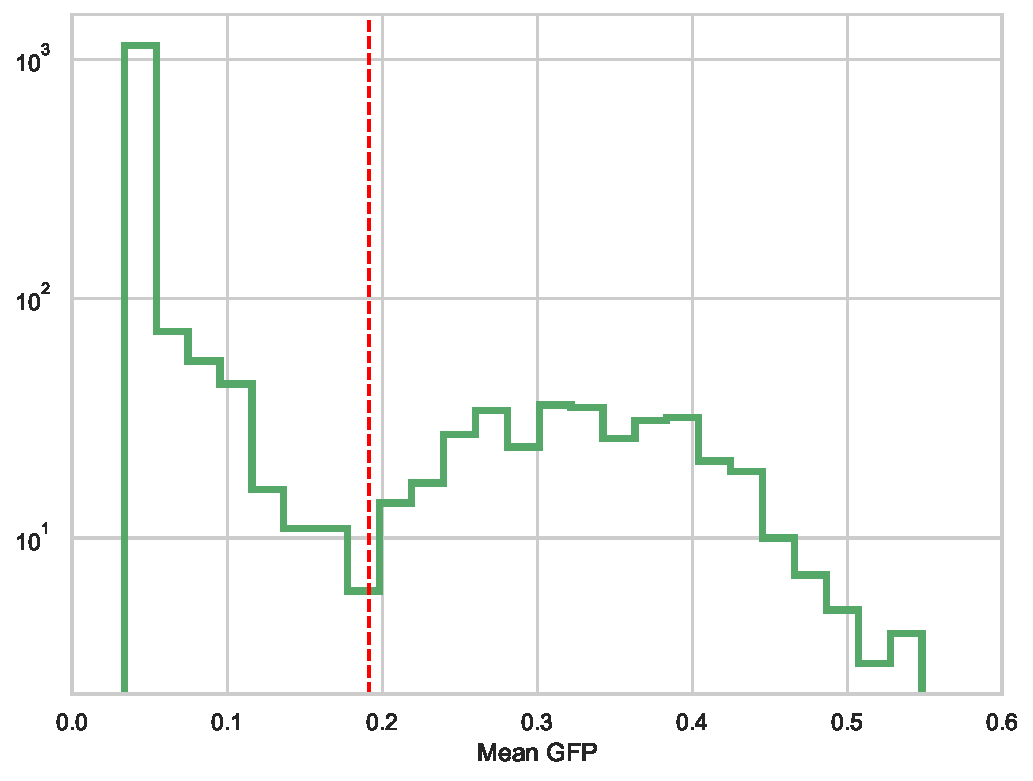
\includegraphics[width=0.85\textwidth]{img/gfp_bimodal.pdf}
\caption{Living and dead Raji cells revealed as distinct modes of a bimodal distribution on mean GFP fluorescence intensity per connected component of cell segmentation output.}
\label{fig:gfp_bimodal}
\end{figure}

\subsection{Object detection system}
\label{subsec:training}

In order to track cell phenotype populations over time, we require a robust object detection system to identify individual cells. The core of our system is a convolutional neural network and is detailed below.

\tikzstyle{block} = [rectangle, draw, fill=blue!20, node distance=2.5cm,
    text width=3.5em, text centered, rounded corners, minimum height=3em]
\tikzstyle{line} = [draw, -latex']

%
%In this section we detail our object detection system and our pre- and post-processing methodology. All code for our system is publicly available\footnote{\texttt{https://github.com/jcboyd/tracking-lymphocytes}}.

\subsubsection{Training as a classifier}

Our preprocessing pipeline is imperfect and does not give a complete annotation of the cell populations as would be required by state-of-the-art detection systems such as \cite{redmon2016you}. We therefore opt for crop-wise training, where the bounding boxes of successfully segmented cells are padded, to create $24\times24$px crops, centered on the cells. Due to the low image resolution, we found this sizing provided sufficient contextual information to the network. Combined with background crops, this amounts to approximately 100,000 training examples in three classes. Samples are given in Figure \ref{fig:crops}.

\begin{figure}[htb]
\centering
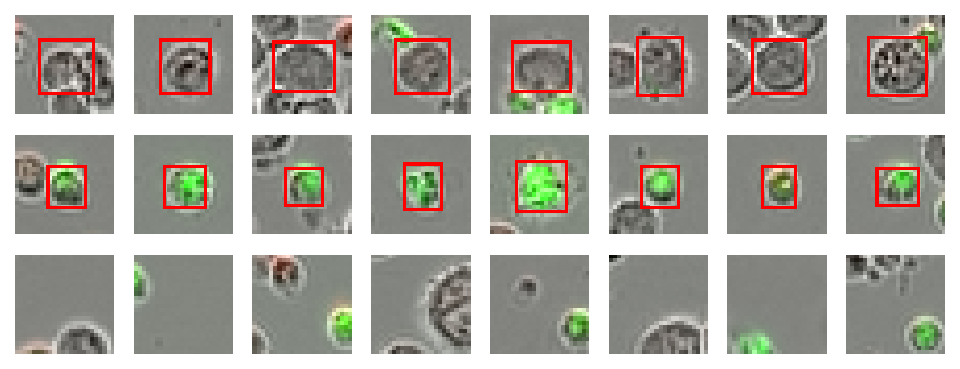
\includegraphics[width=\textwidth]{img/crops.pdf}
\caption{Samples of living Raji cells (top), dead cells (middle), background (bottom) annotated with bounding boxes. Fluorescence is included for clarity only and is not used in training.}
\label{fig:crops}
\end{figure}

% the following design: two consecutive blocks of $3\times3$ convolution $\to$ batch norm $\to$ ReLU activation; a $2 \times 2$ max pooling; two further blocks of $3\times3$ convolution $\to$ batch norm $\to$ ReLU activation; a final $1\times1$ convolutional layer with softmax activation.

Our network architecture is detailed in Table \ref{table:nn}. All weighted layers have a ReLU activation, except Output$_o$ and Output$_c$, which have softmax activations, and Output$_b$, which remains linear. The convolutions are all valid, and a $24\times24$px input image is reduced to $1\times1$px by the final layer. We implement this network in the \texttt{Keras} deep learning framework\cite{chollet2015keras} and all code for our system is publicly available\footnote{\texttt{https://github.com/jcboyd/detecting-lymphocytes}}. We train the network with stochastic gradient descent with learning rate $5 \times 10^{-3}$ and Nesterov momentum $(\mu = 0.9)$. Mini-batches of size 128 are sampled stochastically and simple data augmentation (horizontal and vertical flipping) is performed on the fly. We regularise the network with batch normalisation \cite{ioffe2015batch} and weight decay ($\lambda = 3 \times 10^{-5}$).

\begin{table}[ht!]
\begin{center}
\begin{tabular}{|c|c|c|c|}
\hline
Layer & Connection & Size & Output ($w \times h \times d$) \\
\hline
Input & - & - & $24 \times 24 \times 1$\\
\hline
Conv$_1$ & Input & ${3\times 3}$ & $22 \times 22 \times 16$  \\
Conv$_2$ & Conv$_1$ & ${3\times 3}$ & $20 \times 20 \times 16$ \\
MaxPool$_1$ & Conv$_2$ & ${2\times 2}$ & $10 \times 10 \times 16$ \\
Conv$_3$ & MaxPool$_1$ & ${3\times 3}$ & $8 \times 8 \times 64$ \\
Conv$_4$ & Conv$_3$ & ${3\times 3}$ & $6 \times 6 \times 64$ \\
MaxPool$_2$ & Conv$_4$ & ${2\times 2}$ & $3 \times 3 \times 64$ \\
Conv$_5$ & MaxPool$_2$ & ${1\times 1}$ & $1 \times 1 \times 128$ \\
Conv$_6$ & Conv$_5$ & ${1\times 1}$ & $1 \times 1 \times 128$ \\
\hline
Output$_o$ & Conv$_6$ & ${1\times 1}$ & $1 \times 1 \times 1$ \\
Output$_c$ & Conv$_6$ & ${1\times 1}$ & $1 \times 1 \times 1$ \\
Output$_b$ & Conv$_6$ & ${1\times 1}$ & $1 \times 1 \times 2$ \\
\hline
\end{tabular}
\end{center}
\caption{Specification of the network architecture. We distinguish three multitask outputs: Output$_o$, the probability of object presence; Output$_c$, the probability of class $c$ given an object; and Output$_b$, the tuple of object width and height.}
\label{table:nn}
\end{table}

Inspired by \cite{redmon2016you}, we formulate a multi-task prediction in which we predict $Pr(o)$, where $o$ indicates the presence of an object in the center of the receptive field and, separately, $Pr(c | o)$, that is, the probability of cell phenotype class $c$ given the presence of an object. These probabilities are combined at inference time (Section \ref{subsubsec:inference}). In addition, our network performs regression on the height $h$ and width $w$ of the bounding box of the cell, measured as a fraction of the crop size from the crop centre. This information is readily available when generating the training set. Note that we make the assumption that our chosen crop size represents a hard maximum on the size of a cell's bounding box, a reasonable simplification for our dataset. Our network is therefore trained to minimise the loss function,

\begin{align}
\mathcal{L}(\mathbf{x}_i, o_i, c_i, w_i, h_i;\theta) = l_{o}(\hat{o}_i, o_i) &+ \mathbbm{1}_{o}^{i}\big[l_{c}(\hat{c}_i, c_i)\big] + \mathbbm{1}_{o}^{i}\big[l_{b}(\hat{w}_i, w_i, \hat{h}_i, h_i)\big],
\end{align}

with respect to model parameters $\theta$, where $l_{o}$ and $l_{c}$ are each a standard cross entropy and $l_b(\hat{w}_i, w_i, \hat{h}_i, h_i) = (\hat{w}_i - w_i)^2 + (\hat{h}_i - h_i)^2$. The estimates $\hat{o}_i, \hat{c}_i$ $\hat{w}_i$, and $\hat{h}_i$ are the network outputs for object presence, object class, and bounding box width and height. The indicator function $\mathbbm{1}_o^i = 1$ when training example $\mathbf{x}_i$ contains an object and $\mathbbm{1}_o^i = 0$ otherwise.

We benchmarked our network as a classifier of cropped cells against a logistic regression trained on features extracted from a pre-trained 50-layer ResNet \cite{he2016deep}, a standard CNN approach in bioimage analysis. In order to do this, we resized our cropped cells to $32 \times 32$px and recorded the final convolutional layer of the ResNet, a vector of dimension $2048$. This baseline achieved an accuracy of $0.83$ on balanced test data, whereas our own network achieved $0.96$. Though deep pre-trained networks are known to be powerful general-purpose feature extractors \cite{sharif2014cnn}, they may also be over-parameterised for many problems \cite{raghu2019transfusion}.
%It does appear, however, the two cell classes are not perfectly separable. This can be due to the imperfections of our ground truth generation, but also that the transmitted light image may not convey the full biological information of the fluorescent signal, as discussed in \cite{ounkomol2018label}.

\subsubsection{Inference as a detector}
\label{subsubsec:inference}

%\begin{figure*}[t!]
%\includegraphics[width=\textwidth]{img/nms.pdf}
%\caption{The processing of a test image. Row-wise then column-wise: phase contrast input image; raw model bounding box predictions; non-maximum suppression post-processing; finally, for comparison, the corresponding full fluorescence image.}
%\label{fig:nms}
%\end{figure*}

\begin{figure}
\centering
\begin{tikzpicture}[node distance=0.5cm, text width=3em, minimum height=3em, font=\tiny]
    % Place nodes
    \node [block, fill=red!20] (data) {Train data $(24\times24)$};
    \node [block, below of=data] (training) {Model training};
    \node [block, left of=training, fill=red!20] (architecture) {FCN architecture};
    \node [block, right of=training, fill=red!20] (classifier) {FCN classifier};
    \node [block, right of=classifier] (inference) {Model inference};
    \node [block, above of=inference, fill=red!20] (test) {Test data $(? \times ?)$};
    \node [block, right of=inference, fill=red!20] (probabilities) {Probability map};
    \node [block, below of=probabilities] (nms) {Non-maximum supp.};
    \node [block, below of=nms, fill=red!20] (bbs) {Bounding box proposals};
%    \node [block, above right of=cluster] (visualise) {Visualise t-SNE};
%    \node [block, below right of=cluster] (crops) {Sample crops};
    % Draw edges
    \path [line] (data) -- (training);
    \path [line] (architecture) -- (training);
    \path [line] (training) -- (classifier);
    \path [line] (classifier) -- (inference);
    \path [line] (test) -- (inference);
    \path [line] (inference) -- (probabilities);
    \path [line] (probabilities) -- (nms);
    \path [line] (nms) -- (bbs);
%    \path [line] (probabilities) -- (visualise);
%    \path [line] (cluster) -- (crops);
\end{tikzpicture}
\caption{Pipeline for training a deployment of a fully convolutional classifier. Training may occur on fixed-sized input ($24 \times 24$)px, but convolutions permit variable-sized inference.}
\label{fig:fcn_pipeline}
\end{figure}

\begin{figure}%
    \centering
    \subfloat[]{{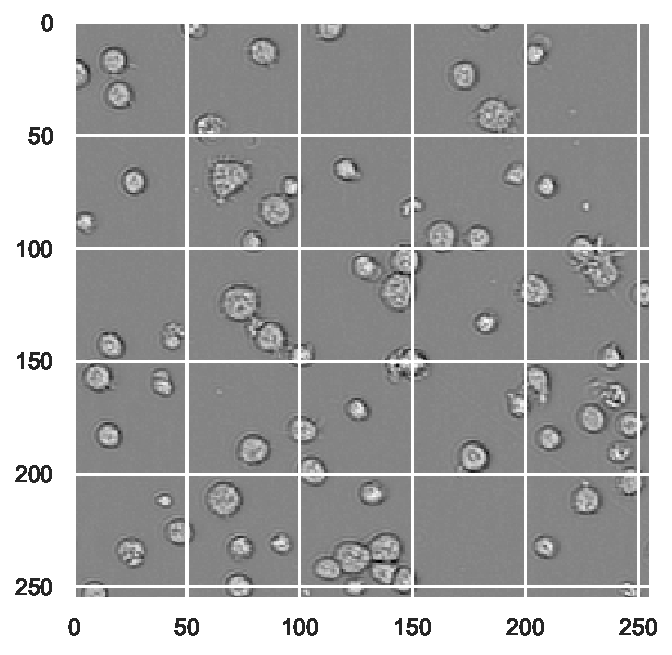
\includegraphics[width=.45\linewidth]{img/nms_input.pdf}}}%
    \qquad
    \subfloat[]{{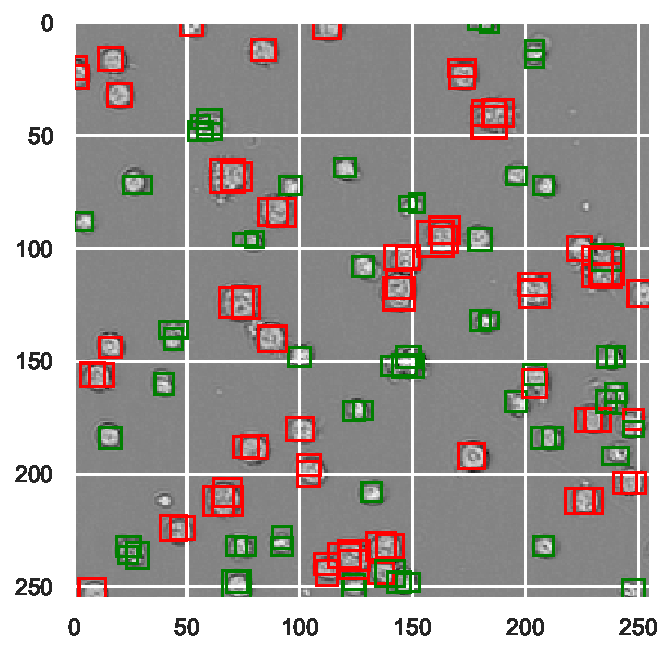
\includegraphics[width=.45\linewidth]{img/nms_raw_detections.pdf}}}%
    \qquad
    \subfloat[]{{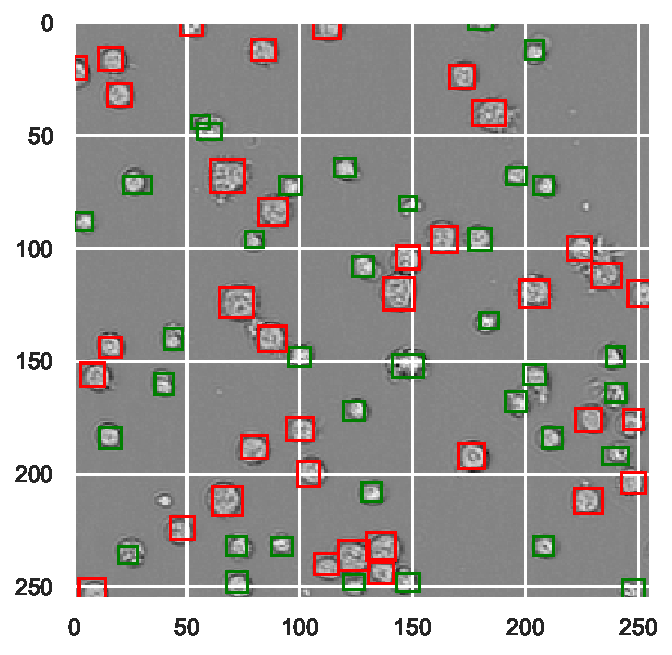
\includegraphics[width=.45\linewidth]{img/nms_post_nms_detections.pdf}}}%
    \qquad
    \subfloat[]{{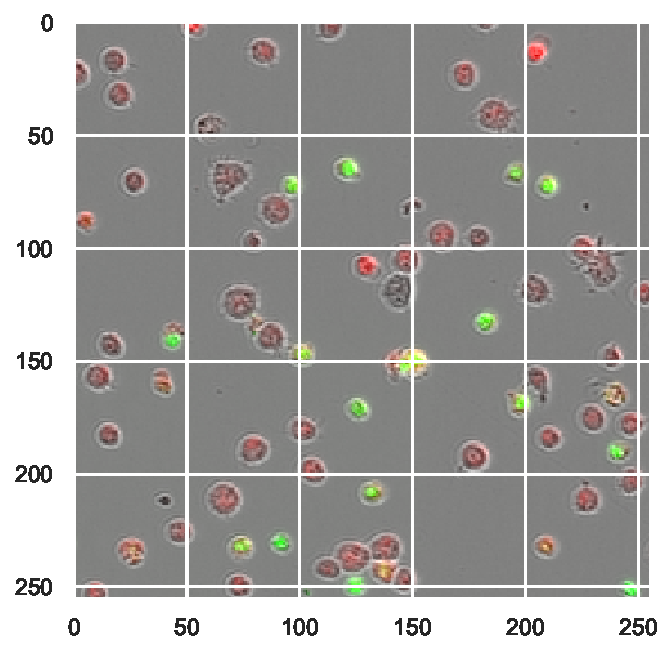
\includegraphics[width=.45\linewidth]{img/nms_full_colour.pdf}}}%
\caption{The processing of a test image: phase contrast input image (a); raw model bounding box predictions (b); non-maximum suppression post-processing (c); finally, for comparison, the corresponding full fluorescence image (d).}
\label{fig:nms}
\end{figure}

Following \cite{sermanet2013overfeat} we designed our network to be \emph{fully convolutional} (FCN). A FCN is capable of performing inference on any size of input, and is extended naturally to object detection. The workflow is specified in Figure \ref{fig:fcn_pipeline}. Thus, once trained on cell crops as a classifier, inference may be performed on an entire image in a single forward pass, producing a map of softmax probabilities at every location in the image. Note that even on CPU, a full $1408 \times 1040$px image is processed by the network in about $1$s.  Fully-convolutional whole-image inference emulates sliding-window detection, albeit without the tremendous inefficiency of executing the model separately at every spatial position. Note that the resolution of the output will depend on the number of pooling layers in the network. For example, our network includes two max pooling layers, hence we make detections at a stride of $4$ across the input image domain.

%We justify our choice of network by benchmarking against against cross-validated SVM (0.89 mean precision and 0.89 mean recall on balanced data) and random forest baseline models (0.89 mean precision and 0.88 mean recall). Note that neither of these can be used efficiently in a sliding window fashion as the CNN can. Moreover, the network outperforms the baselines (0.96 mean recall and 0.96 mean precision)



%\subsection{Calibrating posterior probabilities}
%
%Class imbalance is a challenge in our application as cells are seeded at different proportions depending on the experiment. Furthermore, cell behaviours such as mitosis often outpace cell death, leading to a trend towards imbalance over the course of the experiment. We require our system to be agnostic with respect to class priors, $\pi_0$ and $\pi_1$ (negative and positive classes).
%
%%\begin{figure}[htb]
%%\includegraphics[width=8.5cm]{img/confusions.pdf}
%%\caption{Confusion matrices for the same classifier on balanced data (left) and unbalanced data (right). The .}
%%\label{fig:confusions}
%%\end{figure}
%
%In Figure \ref{fig:confusions} we see how errors accumulate when a network trained on balanced data is confronted with an imbalanced dataset. Although the classifier has 95, $\pi_0 >> \pi_1$ leads to an abundance of false positives (116), a  . To mitigate this. effect \cite{dal2015calibrating} propose a calibration formula with posterior probabilities. Let denote $C_0$ and $C_1$ represent regions of feature space for class 0 and class 1 respectively where, $C_0 = \big\{\mathbf{x} : p(C = c_0 \ | \ \mathbf{x}) \geq \rho)\big\}$ and, $C_1 = \big\{\mathbf{x} : p(C_1 \ | \ \mathbf{x}) \leq \rho)\big\} = \big\{\mathbf{x} : p(C_0 \ | \ \mathbf{x}) \geq 1 - \rho)\big\}$ for some probability level $\rho$. Now define the set, $\mathcal{M} = C_0 \cap C_1 = \big\{\mathbf{x} \ : \ p(C_0 \ | \ \mathbf{x}) = \rho\big\}$. This defines a particular probability contour between the classes e.g. a decision boundary. Denote class priors $\pi_0 = p(C_0)$ and $\pi_1 = p(C_1)$. By Bayes' theorem,
%
%$$p = \frac{\pi_0p(\mathcal{M} \ | \ C_0)}{\pi_0p(\mathcal{M} \ | \ C_0) + \pi_1p(\mathcal{M} \ | \ C_1)}$$
%
%where $p = p(C_0 \ | \ \mathcal{M})$ is the posterior probability. If the priors change, the conditional probabilities do not change, but the posteriors do,
%
%$$p' = \frac{\pi_0'p(\mathcal{M} \ | \ C_0)}{\pi_0'p(\mathcal{M} \ | \ C_0) + \pi_1'p(\mathcal{M} \ | \ C_1)}$$
%
%where $p' = p(C_0 \ | \ \mathcal{M}, \pi_0'$, $\pi_1')$ given adjusted priors $\pi_0'$ and $\pi_1'$. Rearranging (1) above gives,
%
%$$p(\mathcal{M} \ | \ C_1) = \frac{\pi_0}{\pi_1}\bigg(\frac{1}{p} - 1\bigg) p(\mathcal{M} \ | \ C_0) $$
%
%Substituting into (2) gives,
%
%$$p' = \frac{\beta p}{\beta p + \beta' - \beta' p}$$
%
%where $\beta = \pi_1/\pi_0$ and $\beta' = \pi_1'/\pi'_0$ i.e. the ratio of positive cases in each rebalancing of the problem. Note that in the particular case of $\pi_0' = \pi'_1$ (balanced dataset), we get,
%
%$$p' = \frac{\beta p}{\beta p + 1 - p}$$
%
%This has the effect of shifting the decision boundary to regions where there is a more even chance of either class.

%\begin{figure}
%\centering
%\begin{tikzpicture}[font=\sffamily]
%\node (A) at (0, 0) {\tiny$(14, 14, 1)$};
%\node (B) at (2, 0) {\tiny$(12, 12, 16)$};
%\node (C) at (4, 0) {\tiny$(10, 10, 32)$};
%\node (D) at (6, 0) {\tiny$(5, 5, 32)$};
%\node (E) at (8, 0) {\tiny$(3, 3, 64)$};
%\node (F) at (10, 0) {\tiny$(1, 1, 64)$};
%\node (G) at (12, 0) {\tiny$(1, 1, K)$};
%\draw [->] (A) -- node [above=0.2cm, align=center] {\tiny{conv$_{3\times 3} \circ \sigma$}} (B);
%\draw [->] (B) -- node [above=0.2cm, align=center] {\tiny{conv$_{3\times 3} \circ \sigma$}} (C);
%\draw [->] (C) -- node [above=0.2cm, align=center] {\tiny{maxpool$_{2\times 2}$}} (D);
%\draw [->] (D) -- node [above=0.2cm, align=center] {\tiny{conv$_{3\times 3} \circ \sigma$}} (E);
%\draw [->] (E) -- node [above=0.2cm, align=center] {\tiny{conv$_{3\times 3} \circ \sigma$}} (F);
%\draw [->] (F) -- node [above=0.2cm, align=center] {\tiny{conv$_{1\times 1} \circ \sigma$}} (G);
%%\draw[-Latex] (A) to (B);
%%\draw[-Latex] (B) to (C);
%%\draw[-Latex] (C) to (D);
%%\draw[-Latex] (D) to (E);
%%\draw[-Latex] (E) to (F);
%%\draw[-Latex] (F) to (G);
%%\draw[-Latex] (C) to (P);
%%\draw[-Latex] (B) to [out=20,in=160] (P);
%\end{tikzpicture}
%\caption{Fully convolutional network architecture. We here illustrate the evolution of the tensor for an input shaped $(14, 14, 1)$, that is, a $14 \times 14$ crop with a single channel. $K$ is the number of classes modeled. The network is engineered to result in a scalar output. Increasing the input size will increase the output size. The function $\sigma$ is the non-linearity, chosen to be a rectified linear unit (ReLU).} 
%\end{figure}

At inference time, the object and conditional class probabilities are combined to give the marginal class probabilities $Pr(c) = Pr(c | o) \cdot Pr(o)$. Note that $Pr(c | \neg o) = 0$. These probabilities are thresholded and pruned with non-maximum suppression (NMS), providing a final detection mask for each class. For the NMS algorithm, we use an intersection over union threshold of 0.35. An example of this procedure is shown in Figure \ref{fig:nms}.

\subsubsection{Smoothing probabilities in time}

Because the cells are relatively stationary, we can improve the prediction of our system by leveraging information across time. We find a simple weighted average of prediction probabilities from consecutive frames, computed prior to NMS, improves overall performance. We thus define the \emph{smoothed} probability $p_{ij}^{(t)} \leftarrow 1/4\cdot p_{ij}^{(t-1)} + 1/2\cdot p_{ij}^{(t)} + 1/4 \cdot p_{ij}^{(t+1)}$ for the probability at image position $(i, j)$ at time $t$. The weights were tuned manually for both performance and parsimony.

%\begin{figure}[htb]
%\includegraphics[width=8.5cm]{img/umap.pdf}
%\caption{UMAP\cite{mcinnes2018umap} visualisations of living (red) and dead (green) Raji cells and background crops (blue) as model inputs (left) and hidden representations (right).}
%\label{fig:umap}
%\end{figure}

%\subsection{Training strategy \#2 - dense detection}
%\label{subsec:dense}

%An alternative strategy to preselecting crops is to train directly on the image itself. We hypothesise that training may attenuate some of the biases connected with crop extraction such as the upsampling, and crude background sampling. Though a good object detection system requires a good constituent classifier, good classification alone may not imply a good object detector in practice. We therefore take a training approach of \emph{dense detection}. To achieve this, we take the segmentation from the ground truth and use the central pixel of each connected component as a marker, which we dilate for robustness, yielding a binary mask of detection markers for each class.
%
%At training time, the regions of the full image are sampled uniformly randomly in mini-batches at a tunable cropping size. We achieved best results for regions of size $28$px $\times 28$px, though a potential source of future work is to explore the effect of varying this size. The output of the network is now a probability tensor, which a softmax preformed at every spatial location. To better account for the class imbalance, we replace the vanilla cross entropy used in the previous training procedure with a focal loss function \cite{lin2018focal}, specifically designed for dense detection. The focal loss for a data sample $\mathbf{x}$ is defined as,
%
%\[
%\mathcal{L}_{focal} = -\alpha_t(1 - p_t)^\gamma\log p_t
%\]
%
%where $p_t = f(\mathbf{x})_t$ is the probability emitted by the model $f$ corresponding to the ground truth label $t$ for example $\mathbf{x}$, $\alpha_t$ is a corresponding weight to address class-imbalance (that we set to the inverse class probability), and $\gamma$ is a tunable hyper-parameter (we set $\gamma = 2$). As such, the focal loss is a sort of modulated cross entropy, down-weighting probabilities close to 1 (those examples about which the model is sure) to dampen their superfluous influence on learning. It therefore embodies a learning strategy analogous to boosting methods, devoting greater attention to hard-to-classify examples. Once trained, the network is used as an object detector as in Section \ref{subsec:crops}.

\subsection{Results}
\label{subsec:object_detection_results}

\subsubsection{Evaluation strategy}
\label{subsubsec:evaluation}

To evaluate our system, we manually annotated three days worth of frames of size $256 \times 256$px from each of two independent experimental replicates, totaling 72 images and approximately 7,000 test object detections. The replicates were chosen to represent different population dynamics: the first exhibits higher levels of cell proliferation; the second exhibits higher levels of apoptosis. We henceforth refer to these two datasets as $A$ and $B$ respectively. The annotations consist of manually annotated bounding boxes around the cells. We make this dataset publicly available along with the images used to train the network\footnote{\texttt{https://zenodo.org/record/3515446}}. Note that despite this manually annotated evaluation dataset, our model is still trained on a ground truth that is automatically generated from the experiment.

%The annotations form a binary mask per object class that we compare with the masks generated by the object detection system.

We score our detections in terms of the distance of the bounding box centers to the ground truth bounding box centers. We define the following metrics:

\begin{itemize}
\item True positive (TP) - a cell is detected in the vicinity of a ground truth cell.
\item False positive (FP) - a cell is detected outside the vicinity of any ground truth cell.
\item False negative (FN) - no cell is detected within the vicinity of a ground truth cell.
\end{itemize}

Here we define vicinity to be $\leq 10$px, the maximum distance a predicted cell center may fall from a ground true center while still falling within the typical cell bounding box ($14 \times 14$px). These metrics are computed per cell class, from which we calculate precision, recall, and $F_1$ scores. Note the $F_1$ score prevails over the commonly used Matthews correlation coefficient as it does not require us to define true negatives (a meaningless quantity in our framework). These are displayed in Tables \ref{table:mitosis} and \ref{table:apoptosis} for test sets $A$ and $B$. We see the effect of smoothing is globally positive, significantly improving the precision of the dead cell class, and giving the highest average $F_1$ scores of $83.86$ for $A$ and $81.19$ for $B$. Note that the results on the dead cell class are markedly worse. We postulate this is due to the class imbalance at test time, as well as the difficulty of discerning individual cells from cell clusters.

\begin{table}[ht!]
\begin{center}
\begin{tabular}{|l|c|c|c|c|}
\hline
Method & Class & Precision & Recall & $F_1$\\
\hline
\multirow{2}{4em}{Without smoothing} & Living & $0.8534$ & $0.8636$ & $0.8585$ \\ 
 & Dead & $0.7179$ & $0.8693$ & $0.7864$ \\
\hline
\multirow{2}{4em}{With smoothing} & Living & $0.8466$ & $0.8883$ & $\mathbf{0.8669}$ \\ 
 & Dead & $0.7702$ & $0.8549$ & $\mathbf{0.8103}$ \\
\hline
\end{tabular}
\end{center}
\caption{Detection performance test set $A$, stratified by object class. Best results in bold.}
\label{table:mitosis}
\end{table}

\begin{table}[ht!]
\begin{center}
\begin{tabular}{|l|c|c|c|c|}
\hline
Method & Class & Precision & Recall & $F_1$\\
\hline
\multirow{2}{4em}{Without smoothing} & Living & $0.9451$ & $0.7778$ & $0.8533$ \\ 
 & Dead & $0.6253$ & $0.8935$ & $0.7357$ \\
\hline
\multirow{2}{4em}{With smoothing} & Living & $0.9447$ & $0.7957$ & $\mathbf{0.8638}$  \\ 
 & Dead & $0.6628$ & $0.8904$ & $\mathbf{0.7600}$ \\
\hline
\end{tabular}
\end{center}
\caption{Detection performance on test set $B$, stratified by object class. Best results in bold.}
\label{table:apoptosis}
\end{table}
 
%We see that the dense detection strategy is overall superior crop extraction approach. We believe this might be due to the ill-calibrated posteriors arising from the biases inherent in the training strategy. The dense detection approach also implicitly allows to view each cell at different shifts, and then to better understand the difference between foreground and background. The cropping strategy has a consistently higher recall, and we suspect the balanced training makes it overly eager to classify objects (at the expense of precision). Nevertheless, there is clear room for improvement for our dense detector, in particular for dead cells. We suspect there is a lot to be gained by tuning the various hyperparameters in our system, something we intend to pursue immediately.

%\begin{table*}[ht!]
%\begin{center}
%\begin{tabular}{|l|c|c|c|c|c|} 
%\hline
%Method & Class & Precision & Recall & $F_1$ \\
%\hline
%\multirow{2}{4em}{Without smoothing} & 0.70 & $\mathbf{0.96}$  & 0.81 & 0.44 \\ 
% & 0.29 & $\mathbf{0.90}$ & 0.44 & 0.44 \\
%\hline
%\multirow{2}{4em}{With smoothing} & $\mathbf{0.91}$ & 0.93 & $\mathbf{0.92}$ & 0.44 \\ 
% & $\mathbf{0.47}$ & 0.74 & $\mathbf{0.58}$ & 0.44\\
%\hline
%\end{tabular}
%\end{center}
%\caption{Comparison of training approaches, stratified by object class. GIVE ABSOLUTE ERROR OF POPULATION CURVES}
%\label{table:results}
%\end{table*}

%
%\begin{figure}[htb]
%\includegraphics[width=8.5cm]{img/sample.pdf}
%\caption{Full fluorescent image crop with live Raji cells in red and dead cells in green (left) compared with a typical sample detection result on phase contrast only (right). A dead cell false positive can be seen in the first row, second column of the grid, and a live cell false negative in the fourth row, third column of the grid.}
%\label{fig:detections}
%\end{figure}

\subsubsection{Tracking population numbers over time}
\label{subsubsec:tracking}
Our detection system is ultimately used to enumerate cell phenotypes over the course of CAR-T experiments. In Figure \ref{fig:populations} we plot ground truth population numbers against the numbers inferred by our system. One can see the increasing number of living cells in Figure \ref{fig:populations}(a), corresponding to increasing amounts of cell division, whereas in Figure \ref{fig:populations}(b), one can see increasing amounts of apoptosis. In the former, our system achieves a mean relative error percentage of $5.95\%$ and $5.56\%$ (resp. living and dead cells) and $5.81\%$ and $5.37\%$ in the latter.

\begin{figure}%
    \centering
    \subfloat[]{{\includegraphics[width=0.9\textwidth]{img/mitosis.pdf}}}%
    \qquad
    \subfloat[]{{\includegraphics[width=0.9\textwidth]{img/apoptosis.pdf}}}%
    \caption{Population curves for manually-annotated test set $A$ (a) and test set $B$ (b), compared with detection system outputs.}
    \label{fig:populations}
\end{figure}

\section{Discussion}
\label{sec:discussion_strategies}

This chapter has shown how fluorescence may be used to generate a robust ground truth for machine learning. It has presented two strategies for quantifying cells from phase contrast images, by leveraging paired fluorescence images. Section \ref{sec:fluorescent_labeling} showed how image-to-image translation models (including a generative adversarial variant) could be used as fluorescent predictors, and could successfully synthesise the fluorescent channels corresponding to a phase contrast microscopy input. Section \ref{sec:object_detection_system} described the training of a neural object detection system and tested it on two manually annotated datasets. An example of how time information can be incorporated into the prediction task was also given. The system can likely be further improved with a more precise and expanded dataset.

Figure \ref{fig:cells_wells} compares the time series derived from applying each method for the complete frames of the first $72$ hours of each time lapse movie in the Raji-only setting. The fields are pooled to obtain a total count for each of the four replicate wells of the Raji-only experiments at each time point. The time series for the detection system are obtained simply by counting bounding boxes as in Section \ref{subsubsec:tracking}. By contrast, the fluorescence predictor requires a more ad hoc approach. The central $1024 \times 1024$px of each frame was cropped and passed through the labeler networks to generate the fluorescent images. A background subtraction was then performed using a mean filter to normalise the intensity levels, before thresholding to obtain a binary mask. The number of non-zero pixels is counted to obtain an index acting as proxy to the total number of cells. Figure \ref{fig:cells_wells} shows a strong correlation between the outputs of the two systems. This is corroborated in Table \ref{table:correlations}. Note that this represents roughly two orders of magnitude more data than the datasets $A$ and $B$ visualised in Figure \ref{fig:populations}.

\begin{sidewaysfigure}
\centering
\includegraphics[width=\textwidth]{img/wells.pdf}
\caption{Comparing cell quantification strategies by accumulation of cell types over time in four well replicates, aggregating over fields of view. The labeling series are normalised to have the same mean as the detection series.}
\label{fig:cells_wells}
\end{sidewaysfigure}

\begin{table}[h]
\begin{center}
\begin{tabular}{|c|c|c|}
\hline
Well & Alive & Dead \\
\hline
A01 & 0.9751 & 0.8935\\
A02 & 0.9851 & 0.8657\\
A05 & 0.9888 & 0.8230\\
A06 & 0.9734 & 0.8840\\
\hline
\end{tabular}
\end{center}
\caption{Correlations between object detection and fluorescence prediction time series for alive and dead Raji cells in four experimental replicates.}
\label{table:correlations}
\end{table}

We therefore see that the approaches are probably on par. The advantage of the labeling approach is that it does not require a handcrafted workflow to generate the ground truth from the experimental data: the ground truth is given by the image pairs themselves. In contrast, the object detection approach requires an ad hoc procedure to derive the cell class label from the fluorescence images. This workflow is particularly easy and can be designed with very basic image analysis methods in the present setting, but for other markers and imaging conditions it would require some re-tuning of parameters. On the upside, the object detection approach directly provides a cell by cell quantification, a level of information which is not directly available in the fluorescence predictions. Indeed, it is less satisfying from the perspective of a biologist to just have a general index that would not allow the assignment of interpretable phenotypic classes to each cell.
